\documentclass[a4paper,12pt]{report}
%\setcounter{chapter}{1}
\renewcommand\thesection{\arabic{section}}
\renewcommand{\contentsname}{Cuprins}
\renewcommand{\figurename}{Figura}
\renewcommand{\tablename}{Tabel}

\setcounter{tocdepth}{6}
\setcounter{secnumdepth}{6}

\usepackage{url}
\usepackage[backend=bibtex,style=numeric,citestyle=numeric,backref=true,sorting=none]{biblatex}
\addbibresource{bibliography.bib}

\usepackage{indentfirst}
\usepackage[nobottomtitles*]{titlesec}

\usepackage{graphicx}
\usepackage[center]{caption}
\usepackage{caption}
\usepackage{subcaption}
\usepackage[export]{adjustbox}
\graphicspath{ {./images/} }



\usepackage[margin=3.9cm]{geometry}
%\usepackage[none]{hyphenat}

\usepackage{mathtools}

\usepackage{listings}
\usepackage{color}
\usepackage{float}

\definecolor{codegreen}{rgb}{0,0.6,0}
\definecolor{codegray}{rgb}{0.5,0.5,0.5}
\definecolor{codepurple}{rgb}{0.58,0,0.82}
\definecolor{backcolour}{rgb}{0.96,0.96,0.96}

\lstdefinestyle{mystyle}{
	backgroundcolor=\color{backcolour},   
	commentstyle=\color{codegreen},
	keywordstyle=\color{blue},
	numberstyle=\tiny\color{codegray},
	stringstyle=\color{codepurple},
	basicstyle=\fontsize{10}{10}\selectfont\ttfamily,
	breakatwhitespace=false,         
	breaklines=true,                 
	captionpos=b,                    
	keepspaces=true,                 
	numbers=left,                    
	numbersep=2pt,                  
	showspaces=false,                
	showstringspaces=false,
	showtabs=false,                  
	tabsize=2
}

\lstset{style=mystyle}

\usepackage{pythonhighlight}

\usepackage{fontspec} % -> LuaLatex
\setmainfont{UT Sans}

\usepackage{setspace}
\setstretch{1.1} % 

\begin{document}
	
	\begin{titlepage}
	
	\vspace*{-3cm}
	\hspace{-2cm}
	
\includegraphics[width=0.8\linewidth]{./images/Logo-UT-MI-SPOT-RO}

	\begin{center}
		\Huge
		
		\vspace{2cm}
		
		\textbf{Lucrare Dizertație}
		
		\vfill
				
		\Large
		\begin{tabular}{ll}
			\textbf{Autor:}&Hanganu Bogdan\\
			\textbf{Coordonator:}&Lect. Univ. Băicoianu Alexandra
		\end{tabular}
		
		\vfill
		
		\Large
		Brașov\\
		Iulie 2022
        
	\end{center}
\end{titlepage}
	\begin{titlepage}
	
	\vspace*{-3cm}
	\hspace{-2cm}
	
\includegraphics[width=0.8\linewidth]{./images/Logo-UT-MI-SPOT-RO}
	
	\begin{center}
		\Huge
		
		\vspace{2cm}
		
		\textbf{Lucrare Disertație}
		
		\vspace{1cm} 
		
		\LARGE Detectarea emoțiilor din perspective multiple
		
		\vfill
		
		\Large
		\begin{tabular}{ll}
			\textbf{Autor:}&Hanganu Bogdan\\
			\textbf{Coordonator:}&Lect. Univ. Băicoianu Alexandra
		\end{tabular}
		
		\vfill
		
		\Large
		Brașov\\
		Iulie 2022
		
	\end{center}
\end{titlepage}
	\newpage
	\tableofcontents
	\newpage
	\pagenumbering{arabic}
	\section{Abstract}
	Text
	\clearpage
	
	\section{Introducere}
	Exemplu cite [\cite{articol_ibima}]. Prima parte a licenței o va reprezenta aplicația Pianify, o aplicație scrisă în C++ și Python având rolul de a recunoaște două instrumente muzicale (pian și trompetă) și a de a le separă într-un format fișier MIDI iar în a doua parte, o serie de experimente și teste care s-au finalizat prin recunoașterea stării rulmentului în funcție de vibrațiile date de acesta. Motivația din spatele acestor două aplicații este dată de pasiunea pentru inteligență artificială, dobândită în decursul anilor de studiu în cadrul facultății precum și de interesul dobândit în domeniul procesării semnalelor în urma perioadei de practică în cadrul firmei Siemens Industry Software .
	
	În capitolele ce urmează voi prezenta principalele tehnici de procesare de semnal, precum și algoritmii de învățare automați utilizați. Arhitectura, tehnologiile utilizate și flow-ul aplicațiilor vor fi explicate în detaliu demonstrând aplicabilitatea acestora.
	
	\clearpage
	
    \section{Inițiere în procesarea semnalelor}
    În domeniul procesării semnalelor, un semnal reprezintă o cantitate care este variabilă în funcție de timp sau spațiu. Aceastea pot fi împărțite în două categorii bine definite \cite{analogVSdigital}: 
    
    \begin{itemize}
    	\item Semnal analog;
    	\item Semnal digital.
    \end{itemize}

    \textbf{Semnalul analog} reprezintă un tip de semnal continuu, care poate fi clasificat în semnal compus și simplu. Analiza semnalelor stabileşte posibilităţile de a reprezenta semnalele prin sume discrete sau continue de funcţii elementare (exponențiale, sinusoidale, treaptă unitate etc). Un semnal simplu poate fi reprezentat de funcția \textbf{sinus}, care nu poate fi descompus. Însă, un semnal analogic compus presupune alcătuirea sa din mai multe funcţii.
    \par
    În cazul \textbf{semnalului digital}, acesta este memorat în mod discret, având formatul datelor în mod binar.
    
    Fiecare tip de semnal, fie analogic sau digital este caracterizat de următorii termeni în funcție de domeniul în care se află \cite{SISW_DSP}. \\
    Mai departe, vom explica o seria de noțiuni care reprezintă termeni cheie în cadrul domeniului timpului:
    
    \begin{itemize}
    	\item Sample rate (Rata de eșantionare) = este numărul de sample-uri (de date) pe care o secundă de semnal ți-o poate oferi. Spre exemplu, dacă un semnal are sample rate-ul de 44.1 KHz, înseamnă că o dată pe secundă sunt adunate 44100 de date care îți oferă informații privind semnalul.
    	\item Window (Fereastra) = reprezintă rezultatul în urma segmentării semnalului în blocuri de lungimi egale
    	\item Block size (Lungimea unei ferestre) = numărul de sample-uri aflate într-o fereastră.
    	\item Frame size (Durata unei ferestre) = durata în secunde a unei ferestre.
    \end{itemize}
    
    Iar în domeniul frecvențelor putem menționa:
    
    \begin{itemize}
    	\item Bandwidth (Lățimea de bandă) = se referă la cea mai mare frecvență captată în urma executării transformatei Fourier
    	\item Spectral Lines (Numărul de linii sprectrale) = frecvențele recunoscute
    	\item Frequency Resolution (Rezoluția frecvenței) = distanță măsurată în Hz între liniile spectrale.
	\end{itemize}
	
	
	În cadrul acestei lucrări, am utilizat semnale acustice, fiind reprezentate de vibrațiile sunetelui propagat prin intermediul aerului. Acest tip de semnal este utilizat în cazul recunoașterii instrumentelor muzicale. În cazul rulmenților, vibrațiile transmise prin intermediul shaft-ului au fost suficiente pentru a face procesarea semnalului și identificarea acestuia. Această  investigație a semnalelor se face cu scopul de a obține informații atât din domeniul timpului cât și din cel al frecvențelor, acestea fiind vitale fazei de preprocesare a semnalului.
	
	Există o diferență clară între domeniul timpului și domeniul frecvențelor, care va fi explicată în capitolul următor, unde vom vorbi despre transformata Fourier precum și despre proprietățile acesteia în cadrul procesării semnalelor.
	%Pentru a putea înțelege diferența dintre domeniul timpului și domeniul frecvențelor, în următorul capitol vom vorbi despre Transformata Fourier, o unealtă matematică folosită adesea în procesarea semnalelor.
	
	\clearpage
	\subsection{Introducere în transformata Fourier}
	Adesea folosită în analiza vibrațiilor, ingineria audio și procesarea de imagini, transformata Fourier este o unealtă matematică care are scopul de a transforma semnalul din domeniul timpului în domeniul frecvențelor, motivul fiind o înțelegere mai în detaliu a frecvențelor \cite{SISW_FT}.
	
	Acest procedeu matematic descoperit de Jean-Baptiste Joseph Fourier (1768-1830) ne sugerează că orice funcție arbitrară poate fi scrisă ca fiind o sumă de sinusuri și/sau cosinusuri (ex. figura \ref{fig:singal_to_sinuses}). Aplicând integrala ($\int $) asupra funcțiilor trigonometrice, putem afla amplitudinea lor .
	
	\begin{figure}[h]
		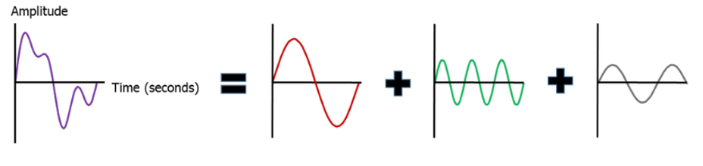
\includegraphics[width=\linewidth]{images/signals.png}
		\caption{Semnal ca fiind o sumă de sinusuri\newline
			\hspace{\linewidth}https://community.sw.siemens.com/s/article/what-is-the-fourier-transform}
		\label{fig:singal_to_sinuses}
	\end{figure}

		
	În general, sunt utilizate două tipuri ale transformatei Fourier :
	 \begin{itemize}
		\item \textbf{Transformata Fourier discretă}, aplică tansformata Fourie pe un număr discret de sample-uri dintr-un semnal. Această tehnică poate fi folosită în general pe orice tip de semnal, având un număr arbitrar de sample-uri.
		\item \textbf{Transformata Fourier rapidă}, este asemănătoare cu procedeul menționat mai sus, singura diferență fiind că numărul de sample-uri care se alege pentru a fi procesat trebuie să fie o putere a lui 2 (spre exemplu, 512, 1024, 2048, 4096 etc), din motive de eficiență computațională. 
	\end{itemize}
	
	\begin{figure}[H]
		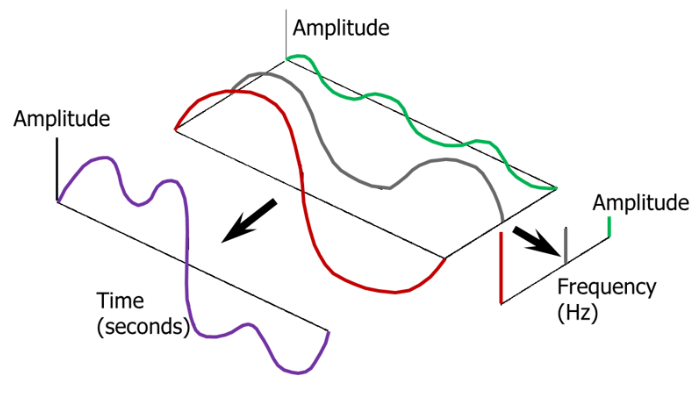
\includegraphics[scale=0.7]{images/FT_time_to_freq}
		\caption{Domeniul frecvențelor \newline
			\hspace{\linewidth}https://community.sw.siemens.com/s/article/what-is-the-fourier-transform}
		\label{fig:signal_to_freq}
	\end{figure}
	
	Pentru a putea exemplifica utilitatea acestui procedeu, ne vom referi la Figura \ref{fig:signal_to_freq}. În această imagine observăm un semnal compus (culoarea mov) care după aplicarea Transformatei Fourier este descompus în trei semnale adiacente, acestea fiind reprezentate de culorile roși, gri și verde având diferite amplitudini. Rezultatul propiu-zis al acestui procedeu matematic este dat de liniile spectrale, reprezentând frecvențele semnalelor descompuse. Faptul că frecvența se măsoară în Hz, ne sugerează periodicitatea semnalului, mai exact, numărul de oscilații pe care îl face acest sinus într-o secundă.
	
	Din punct de vedere matematic, transformata Fourier este :
	\begin{equation}
		\label{ft_equation}
		S_x(f) = \int_{-\infty}^{+\infty} x(t)e^{-j2 \pi ft} dt
	\end{equation}
	unde $S_x(f)$ reprezintă frecvența măsurată în Hz iar $x(t)$ este semnalul în domeniul timpului. Rezultatul acestei operații este un număr complex (spre exemplu $a + bj$ este un număr complex întrucât a reprezintă partea reală iar b partea imaginară). Dar de ce ?
	
	Rezultatul obținut în urma aplicării transformatei Fourieri este o serie de numere, unde fiecare valoare din această serie corespunde frecvenței, amplitudinii și fazei semnalului. Numerele complexe utilizate în cadrul acestei teoreme au forma fel ca cele menționate mai sus în exemplu (deseori făcându-se referire la acest tip de număr cu litera \textbf{z}).
	
	Aceste numere conțin informații referitor la amplitudinea și faza semnalului inițial, aflat în domeniul timpului.
	
	Astfel, există următoarea relația între partea imaginară și partea complexă a unui astfel de număr, din punct de vedere al trecerii din domeniul timpului în cel al frecvențelor :
	\begin{align}
		\label{ft_amplitude_phase}
		ampl &= \sqrt{a^2 + b^2} &  phase = atan(\frac{b}{a})
	\end{align}
	Utilizând aceste forumule, putem afla amplitudinea precum și perioada semnalului într-un anumit punct. Aceste două concepete ne sunt de folos deoarece, în general, o analiză destul de profundă a semnalelor (fie ele acustice, electromagnetice etc) se pot face prin plotarea acestor rezultate. În sine, graficele obținute în urma plotării celor două noțiuni se numesc informații spectrale.
	
	Deoarece infomațiile fazei sunt păstrate în urma executării acestui procedeu, poate apărea în discuție și inversa transformatei Fourier, ideea de a transforma semnalul înapoi din domeniul frecvențelor în domeniul timpului.

	\bigbreak
	
	Transformata Fourier produce un spectru dublu. Un spectru dublu constă atat în frecvențe negative cât și în cele pozitive (referire la teorema lui Nyquist). Deoarece limitele numerice ale tranformatei Fourier trec de la numere negative la numere pozitive, la fel trece și limita numerica a distanței reprezentate de frecvențe. Amplitudinea maximă a acestui dublu spectru este jumătatate din amplitudinea maximă din semnalul aflat în domeniul timpului. Din convenție, sistemele digitale de achiziție de date specializate pe semnale/vibrații nu iau în considerare frecvențele negative când aplică metode care sunt legate de transformata Fourier. În schimb, aplitudinile pozitive sunt dublate pentru a compensa acest lucru.
	
	Pentru început, vom enumera și discuta funcțiile elementare clasice: 
	\begin{itemize}
		\item Funcția sinus; Funcția sinus este cea mai fundamentală componentă a Transformatei Fourier. Transformata Fourier a unei funcții sinus produce o singură amplitudine împreuna cu faza corespunzătoare la o singură poziție, indicată de frecvență.
		\item Sinus descrescător/crescător; Dacă amplitudinea unui sinus scade, frecvența va fi reprezentata de o "pantă". Cu cât funcția sinus va descrește tot mai repede, cu atât panta va deveni din ce în ce mai abruptă.
		\item Funcția pătrată; Aceasta are în domeniul frecvențelor un număr impar de armonice, care descrește cu o parte fixă din amplitudine.
		\item Un impuls; Transformata fourier a unui impuls (băț) are o amplitudine relativ plată pe tot spectrul frecvențelor. Aceasta sunt adesea folosite în scopuri de testare.
		\item Semnal constant; Un semnal care este constant și are o valore "offset" față de amplitudinea zero, nu are nicio frecvență. Rezultatul ăn urma aplicării transformatei Fourier are frecvența la zero Hz.
	\end{itemize}
	
	Datorită transformării din domeniul timpului în cel al frevcențelor, transformata Fourirer devine o unealtă puternică folosită în cadrul analizei semnalelor. Putem identifica frecvențele predominante precum și degradarea lor în funcție de timp. Acestea fiind spuse, vom prezenta câteva domenii în care acest procedeu are un rol esențial:
	\begin{itemize}
		\item Analiza muzicală; Când analizăm în general sunetele, amplitudinea din spectrul frecvențelor este afișată în decibeli (o cantitate logaritmică). Decibelii sunt considerați a fi o bună reprezentare a modului în care un om percepe sunetul, acela fiind logaritmic.
		\item Analiza echipamentelor rotative precum rulmenți; Transformata Fourier poate fi folosită pentru a identifica un potențial rulment stricat. Fiecare componentă a unui rulment (cursa interioară, cursa exterioară, bilele) intră în contact una cu cealaltă la un interval regulat în cadrul unei rotații. Starea unui rulment poate fi analizată monitorizând vibrațiile acestuia utilizând un senzor de vibrații.
		\item Filtrarea audio; Transformata Fourier poate identifica acele frecvențe care acoperă semnalul(zgomotul) pe care dorim să îl analizăm.
		\item Vibrațiile și zgomotele unui motor; În cadrul acestui domeniu, transformata Fourier este folositoare deoacere multe componente din alcătuirea unui motor emit armonice unice. Prin identificarea acestor componente, putem interpreta diferite vibrații și să stabilim dacă motorul se află în parametrii normali sau nu.
	\end{itemize}

	\newpage
	\subsection{Transformata Fourier pe termen scurt (STFT)}
	Adesea în practică, semnalele variază destul de mult în domeniul timpului, fiind dificilă interpretarea lor dintr-o singură operație. O tehnică asemănătoare cu transformata Fourier reprezintă Short Time Fourier Transform (STFT), care vine în sprijinul asigurării rezoluției frecvențelor. 
	
	Această tehnică des utilizată nu este decât aplicarea succesivă a transformatei Fourier pe bucăți egale din punct de vedere a sample-urilor. Un termen nou care apare în cadrul acestei tehnici îl reprezintă noțiunea de "windowing", însemnând că segmentele se vor intercala, ajungând ca fiecare segment să conține câteva informații din segmentul anterior. Motivul din spatele aplicării acestei tehnici este susținut de eficiența computațiilor cât și de obținerea frecvențelor într-un mod mai determinist. Această metodă se poate ilustra în Figura \ref{fig:windowing} unde se exemplifică procesul prin care semnalul de intrare este împărțit în segmente, observându-se în detaliu fenomenul de "windowing".
	
	\begin{figure}[H]
		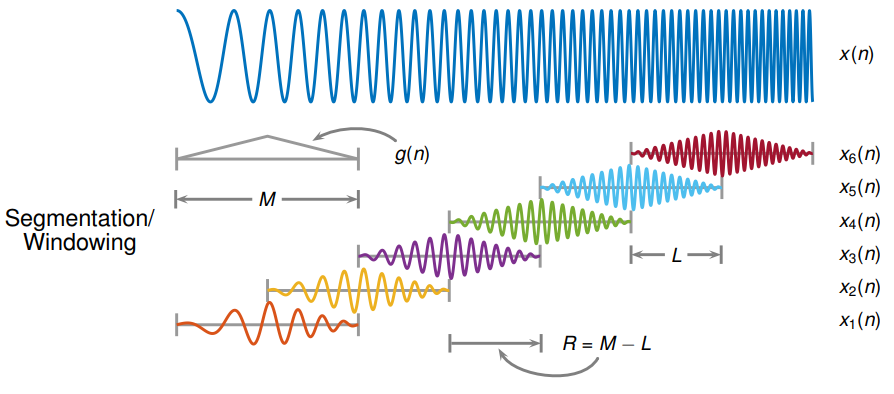
\includegraphics[width=\linewidth]{images/windowing.PNG}	
		\caption{Domeniul frecvențelor \newline
			\hspace{\linewidth}https://nl.mathworks.com/help/signal/ref/stft.html}
		\label{fig:windowing}
	\end{figure}
	
	Un mod util de a reprezenta segmentarea semnalului într-un ansamblu vizual o reprezintă \textbf{spectograma}, denumită și \textbf{"waterfall"}. Practic, într-un spațiu de coordonate XOY, o axă va reprezenta domeniul timpului, cealaltă axă frecvențele iar culorile, amplitudinea semnalului în acel punct. Intensitățiile culorilor vor însemna cât de puternice vor fi frecvențele. În exemplul de mai jos, Figura \ref{fig:spectogram}, avem spectograma unui clip audio care conține un om vorbind. Putem observa cum cele mai puternice frecvențe aparțin intervalului (0,1000) Hz. Folosim acest tip de plotare pentru a observa schimbările frecvențelor și amplitudinilor în raport cu domeniul timpului.
	
	\begin{figure}[h]
		\begin{center}
			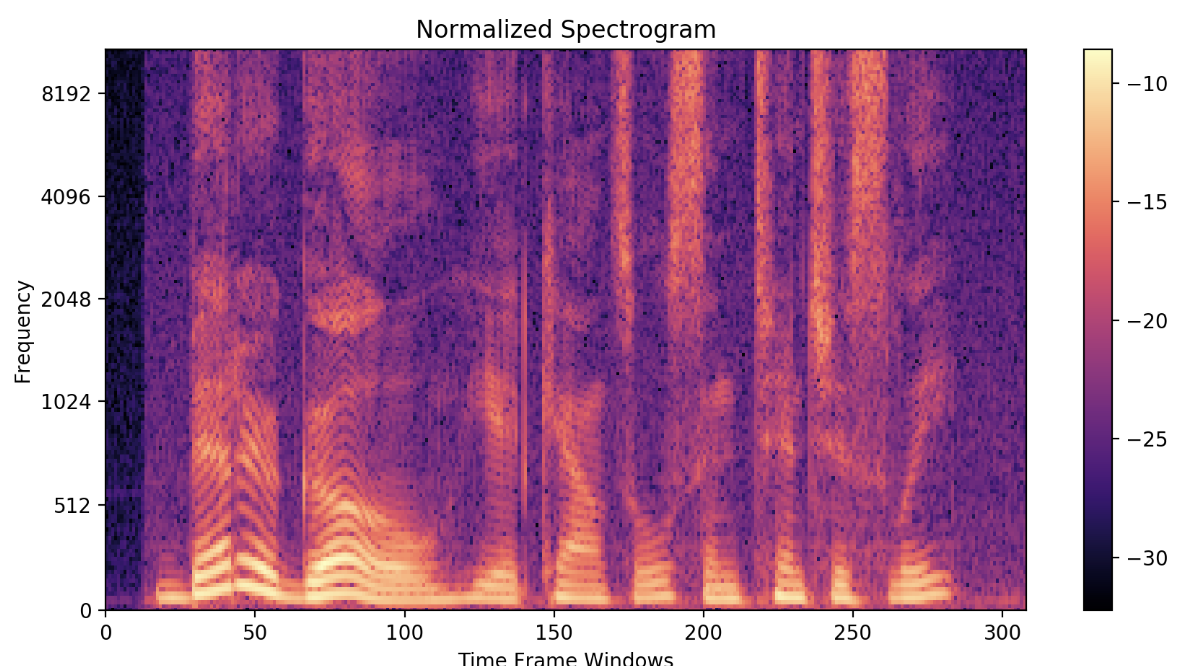
\includegraphics[scale=0.3]{images/spectogram.PNG}
		\end{center}
		\caption{Spectogramă \newline
			\hspace{\linewidth}https://towardsdatascience.com/understanding-audio-data-fourier-transform-fft-spectrogram-and-speech-recognition-a4072d228520}
		\label{fig:spectogram}
	\end{figure}
	
	Procedeele discutate mai sus au o arie de aplicabilitate destul de vastă, însă, pentru aplicațiile pe care urmează să le dezvoltăm există necesitatea definirii unor alte componente. Tranformata Fourier împreună cu variațiile acesteia ne oferă strict informații privind frecvența, amplitudinea/magnitudinea etc însă nicio informație privind apartenența semnalului de o anumită categorie. În sprijinul cerințelor noastre, vom vorbi despre Mel-frequency cepstral sau MFC, o tehnică de extragere a unor trăsături, des utilizată în recunoașterea vocală.	
    
    \clearpage
    \subsection{Coeficietenții Mel-frequency cepstral}
    Așa cum a fost definit mai sus, MFC este o tehnică de extragere a trăsăturilor dintr-un semnal (în general audio), adesea utilizată în recunoșterea vocii umane \cite{MFCC_PC}. Punctul de start în cadrul acestei metode este reprezentat de către \textbf{cepstrum}, care reprezintă o secvență numerică oferindu-ne informații referitoare frame-ului analizat, fiind foarte asemănătoare cu o secvență autocorelată. Aceștia sunt obținuți în urma aplicării inversei transformatei Fourier asupra puterii semnalului, adus într-o scală logaritmică. Din punct de vedere matematic, putem descrie astfel:
    
    \begin{equation}
    \label{cepstrum_formula}
   	 	IDFT(log(P(k))) \rightarrow C(n)
    \end{equation}
    
    Un aspect major care trebuie amintit reprezintă transformarea semnalului în scala Mel. Acestă nouă scală percepe frecvențele într-un mod logaritmic, fiind foarte asemănător cu modul în care un om percepe sunetul. Urechea umană este de așa natură încăt să poată distinge foarte ușor schimbările semnalelor acustice emise la frecvențe joase vs de cele înalte. Altfel spus, vom puteam distinge cu ușurință sunetele care au o frecvență joasă (spre exemplu, un robinet deschis are o frecvență de aproximativ 250 Hz) față de cele înalte (un fluier cu ultrasunete folosit în dresajul câinilor, având o frecvență cuprinsă între 2000 și 25000 Hz).
    \\
    \bigbreak
    Pentru a putea converti în scala Mel putem utiliza formula de mai jos: \ref{to_mel_scale}:
    \begin{equation}
    \label{to_mel_scale}
    	m=1125 * ln(1+f/700)
    \end{equation}
    
     unde f reprezintă frecvența pe care dorim să o transformăm iar m rezultatul în scala mel (adesea făcându-se referire ca mels). În sensul invers al operaților, se folosește formula:
     
    \begin{equation}
    \label{from_mel_scale}
    	f=700*(10^{\frac{m}{2595}} -1)
    \end{equation} 
    
    Pentru extragerea coeficienților MFC (MFCC), suntem nevoiți să reproducem următorii pași:
    \begin{itemize}
    	\item Împărțim semnalul în ferestre;
    	\item Estimăm intesitatea semnalului pentru fiecare fereastră (periodogram);
    	\item Filtrăm rezultatul utilizând filtre de tip Mel;
    	\item Aplicăm operația log peste rezultat;
    	\item Decorelăm semnalul utilizând Discret Cosine Transform (DCT);
    	\item Păstrăm statistic un număr de coeficienți (în jur de 10-20), în funcție de degradarea sunetului în timp.
    \end{itemize}

 	Motivația din spatele utilizării acestui set de pași este următoarea: vom fragmenta semnalul în segmente (pentru că pe perioade mici informația nu variază foarte mult), făcând astfel posibilă reținerea unui număr cât mai mare de informați legate de semnal. Următorii doi pași sunt justificați de maniera în care un om percepe sunetul. Cum a fost precizat mai sus, un om nu poate discerne două sunete din punct de vedere al frecvenței dacă aceste sunete sunt la o distață destul de mică. Pentru această situație particulară, putem utiliza proprietățile filtrelor Mel (Figura \ref{fig:mel_scale}). 
	
	\begin{figure}[H]
		\begin{center}
			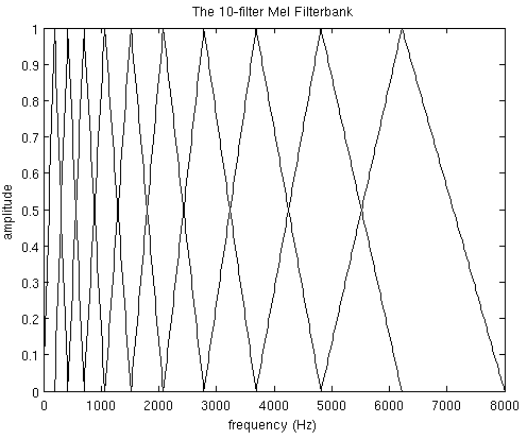
\includegraphics[scale=0.3]{images/mel_filterbank.PNG}
		\end{center}
		\caption{Spectogramă \newline
			\hspace{\linewidth}http://practicalcryptography.com/miscellaneous/machine-learning/guide-mel-frequency-cepstral-coefficients-mfccs/}
		\label{fig:mel_scale}
	\end{figure}
	
	Filtrul Mel, așa cum se observă în Figura \ref{fig:mel_scale}, este destul de îngust la început și devine din ce în ce mai larg pe măsură ce crește frecvența. Astfel, pe masura ce frecvența crește, vom reține mai puțină informație privind frecvențele din semnal datorită energiei semnalelor care devine din ce în ce mai slabă. Faptul că se aplică operația de logaritmare asupra datelor este din nou motivată de percepția sunetului de către om, aceea find una logaritmică. În mod normal, la aplicarea succesivă a diverselor filtre se obțin secvențe de coeficienți care sunt corelate. Acest lucru semnifică modificările dintr-o secvență se propagă și în celelate secvențe ulterioare. Nu este de dorit acest lucru. De aceea vom folosi DCT, pentru a decorela datele și a obține cât mai multe informații. Faptul că vom păstra doar un număr mic de coeficienți este justificat de degradarea sunetului.
	
	\bigbreak
	
	Având aceste metode de procesare a semnalului digital, putem considera cea din urmă metodă de procesare, MFC, ca fiind cea pe care o vom folosi în special pentru antrenarea rețelelor neurale. În capitolul următor, vom descrie cateva generalități despre  inteligența artificială apoi vom insista pe metodele de machine learning utilizate, modelele folosite și vom da câteva caracteristici despre seturile de date întrebuințate în cele două aplicații.
	
    \clearpage
    \section{Inteligența artificială}
     Inteligența este definită ca fiind "abilitatea unui sistem de a se adapta astfel încât să își poată îndeplini scopurile (David Fogel). Din punct de vedere a mașinăriilor, inteligența artificială înfățișează abilitatea unei mașinării programate de a simula inteligența umană. Putem deduce din aceste fraze că acest domeniu aduce în lumea ingineriei software abilitatea mașinăriilor de a lua decizii fără nevoia ca om a acționa în acest scop.
     
     Acest domeniu constituie o înglobalizare a tot cea ce reprezintă abilitatea unei mașinării de a se adapta în diferite situații. Așa cum se observă și în Figura \ref{fig:ai_ml_dl}, inteligența artificială cuprinde machine learning și deep learning.
     
     \begin{figure}[H]
     	\begin{center}
     		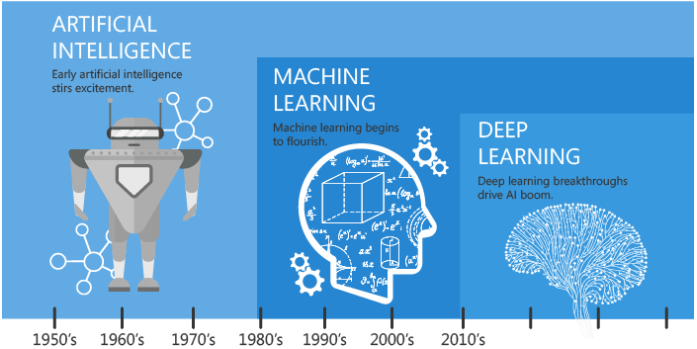
\includegraphics[scale=0.5]{images/AI_ML_DL.PNG}
     	\end{center}
     	\caption{AI vs ML vs DL \newline
     		\hspace{\linewidth}https://www.7wdata.be/big-data/ai-vs-machine-learning-vs-deep-learning/}
     	\label{fig:ai_ml_dl}
     \end{figure}
 
 	 Învățarea automată (machine learning) este un domeniu al informaticii care se ocupă cu învățarea unor sisteme complexe să execute anumite sarcini fără ca aceasta să fie programate în mod explicit să le facă. Principalul obiectiv al învățării automate este acela de a construi algorimiti capabili de a face predicții pe anumite seturi de date. Acești algormiti sunt speciali, deoarece ei nu urmează anumite linii de ghidare ale programarii clasice (unde fiecare linie de instrucțiune trebuie executată cu succes), ci se antrenează pe anumite date pe care le cunoaște deja răspunsurile. Pe baza antrenamentului efectuat, un astfel de algoritm va deveni capabil să ofere predicții destul de apropiate de rezultatul dorit, pe seturi noi de date, necunoscute apriori lui. 
    
   	 Pe scurt, când vorbim despre machine learning, ne gândim la capacitatea unor algoritmi de a identifica anumite tipare în setul de date, de a le învața și de a le putea recunoaște din nou în alte seturi date. Acest domeniu al învățării automate a evoluat în timp, devenind foarte popular datorită divereselor probleme care s-au abordat. Aceste model au fost construite astfel încât să fie capabile să abordeze problemele. Specific acestor algoritmi, putem descrie următoarele tipuri de învățare \cite{supervised_unsupervised} :
   	 
   	 \begin{itemize}
   	 	\item \textbf{Învățare supervizată}, cea în care datele de intrare sunt categorizate astfel încat modelul se antrenează pe baza unui set de date. Spre exemplu, în cazul regresiei, să presupunem că vom încerca să mapăm funcția $y = f(x) $. Scopul regresiei este acela de a aproxima o ieșire (y) cât mai bine astfel încat pentru un set nou de date sa se poata prezice o iesire corecta. În cazul clasificării, scopul algoritmului este de a învăța datele precum si categoria din care face parte, mai apoi, de a putea identifica daca noi date fac parte din cateforiile corespunzatoare.
   	 	
   	 	\item \textbf{Învățare nesupervizată}, cea în care avem datele de intrare, dar nu și o ieșire asociată acestora. Scopul acestui tip de învățare este acela de a descoperi structuri/pattern-uri în seturile de date. Acest tip de învățare la rândul ei se poate clasifica în: 
   	 	\begin{itemize}
   	 		\item Clustere, unde vrem să grupăm datele care au trăsături comuneș
   	 		\item Asociere, în care dorim descoperirea unor reguli care se aplică asupra datelor .
   	 	\end{itemize}
    	
    	\item \textbf{Învațare prin "întărire"} (reinforcement), unde se presupune ca un agent inteligent inavta sa execute un anume set de pasi. Acest agent va deveni capabil să îndeplinească sarcini complexe, comportamentul lui fiind "coordonat" pe baza unor recompense. Acest tip de învățare este adesea utilizată în jocurile video, unde la fiecare pas se poate discuta despre o miscare optimă.
   	 \end{itemize}
    
    Deep learning nu este altceva decât un subset al machine learning-ului care se specializează în general pe arhitecturile de tip rețele neurale multistrat. Construirea unor arhitecturi cu mai multe straturi, spre exemplu un ConvNet, fac posibilă învățarea unor seturi de date mai complexe (ex. imagini), prin găsirea unor pattern-uri care sunt greu de identificat de către modelele obișnuite, obținând astfel rezultate mai bune.
    
   	Aplicabilitatea inteligenței artificiale este în continuă dezvoltare, atingand inclusibv domenii care la prima vedere nu ar avea nevoide de automatizare. Spre exemplu, un domeniu în care acest concept este utilizat poate fi cel al mașinilor care se conduc singure ("Autonomous Driving"), în care cu ajutorul rețelelor neurale (în general cele convoluționare), detectarea obiectelor (computer vision) și procesarea imaginilor, o mașină poate exercita un astfel de comportament. În domeniul medical, putem aminti de identificarea celor două tipuri de tumori: benigne (cele necanceroase, motiv mic de îngrijorare) și maligne (precanceroase, netrate la timp aduc cancer). 
   	
   	În cadrul acestei licențe, scopul utilizării inteligenței artificiale este motivat prin definirea categoriilor instrumentelor muzicale (procesarea de semnale audio) precum și determinarea stării unor rulmenților (prin intermediul studierii vibrațiilor produse). Pe baza coeficienților MFC (discutați în cadrul capitolului de procesare a semnalelor), vom putea antrena diferite rețele neurale, vom putea să le comparăm rezultatele și vom putea să alegem acei hiperparametrii care oferă o acuratețe cât mai mare. 
   	
   	În secțiunile următoare vom prezența minimalist Multilayer Perceptron (Perceptronul Multistrat), rețele neurale convoluționale, rețele autoencoder, precum și două tehnici de "tunning" a hiperparametrilor (grid search și random search). Mai apoi, vom discuta despre seturile de date utilizate în cadrul celor două aplicații, precum, și oferirea unor mici detalii legate de o tehnică de reducere a dimensiunilor numită Principal Component Analysis (PCA).
   	
   	\clearpage
   	\subsection{Perceptronul multistrat}
   	Perceptronul multistrat este o rețea neurală de tip feedforward, alcătuită din mai mulți neuroni care permit funcții de activare neliniare \cite{ia_sasu}. O astfel de rețea este alcătuită în general din minim 3 straturi:
   	
   	\begin{itemize}
   		\item \textbf{Un strat de intrare}, neavând rol computațional ci doar de a prealua intrările și de a le mapa;
   		\item \textbf{Minim un strat ascun}s alcatuit din neuroni;
   		\item \textbf{Un strat de ieșire}, unde sunt prezise clasele/estimările.
   	\end{itemize}
   
    Urmarind versalitate și invatare cat mai corecta a petttern-urilo dintrun set de date, in ambele aplicatii trata in aceasta lucrare am folosit MLP. Fiind o rețea de tipul feedforward, putem enumare doi pași care se întâmplă în cadrul procesului de antrenare: pasul de propagare înainte și pasul de propagare înapoi (backpropagation). În cadrul primului pas, se aplică o funcție de activare non-liniară pe fiecare strat acelor neuroni care sunt cei mai "excitați" cu scopul activării neuronilor din următorul strat (funcția de activare poate fi diferită de la strat la strat). Am ales funcția RELU (Rectified Liniar Unit) care este definită ca fiind:
   
   \begin{equation}
   \label{relu_formula}
  		y = max(0,x)
   \end{equation}
   
   Pe ultimul strat al rețelei, am folosit funcția de activare softmax (fiind o problemă de clasificare):
   
   \begin{equation}
   \label{softmax_formula}
   		softmax(x) =\frac{ e^x}{\sum e^x}
   \end{equation}
   
   În cadrul propagării înapoi, utilizând funcția de cost Cross Entropy:
   
   \begin{equation}
   \label{cross_entropy_formula}
	   Loss= -\frac{1}{n}\sum log(y')y
   \end{equation}
   (unde n = numărul de date de intrare, y' = categoria prezisă, y = categoria adevarată), vom calcula gradientul și vom actualiza ponderilor (adesea făcându-se referie ca weight) în fiecare neuron de pe fiecare strat. Acest set de instrucțiuni se vor executa de n ori (numărul de epoci) sau până când nu există o diferență majoră din punct de vedere al funcției de cost, de la epocă la epocă (convergență) . În fiecare epocă, datele se vor împărți în batch-uri, având un număr mai mic de date, care se vor propaga prin rețea, cauzând actualizarea ponderilor mai eficientă din punct de vedere computațional.
   
   \begin{figure}[H]
   		\begin{subfigure}[b]{0.57\textwidth}
   			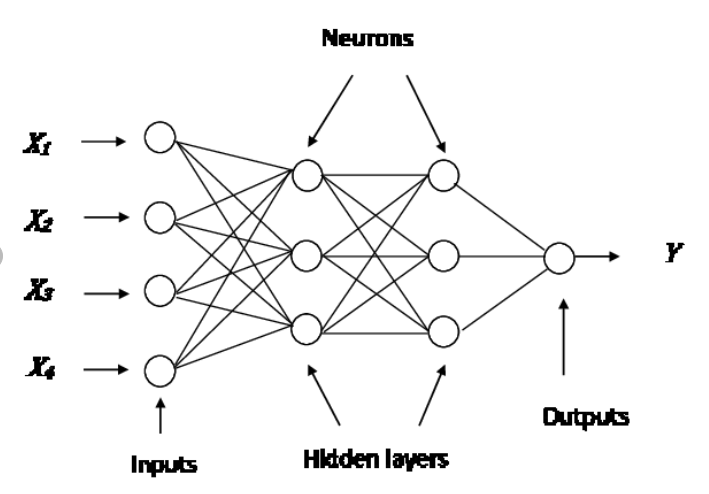
\includegraphics[width=\textwidth]{images/mlp.PNG}
   			\caption{Exemplu de arhitectură}
   			\label{fig:arhitectura}
   		\end{subfigure}
   		\hfill
	   	\begin{subfigure}[b]{0.57\textwidth}
	   		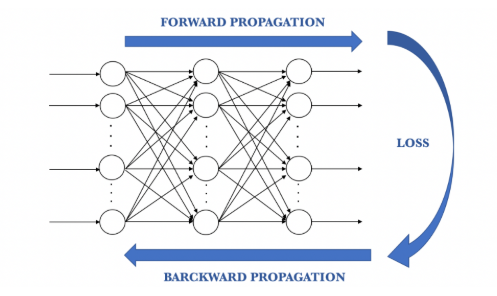
\includegraphics[width=\textwidth]{images/back_propagation.PNG}
	   		\caption{Flow-ul antrenării}
	   		\label{fig:flow_antrenare}
	   	\end{subfigure}
   	\caption{Perceptronul multistrat}
   	\label{fig:arhitectura_flow}
   \end{figure}

    În Figura \ref{fig:arhitectura} putem observa o arhitectură de perceptron multistrat alcătuită din 4 straturi , dintre care 2 sunt ascunse. Primul strat este cel de intrare, în care vom primi datele, urmând apoi să se execute pasul de propagare înainte (cum este prezentat în Figura \ref{fig:flow_antrenare}). În funcție de rezultatul obținut la calcularea erorii, în pasul de propagare înapoi, se vor actualiza ponderile rețelei.
   
    \clearpage
    \subsection{Rețele neurale convoluționale}
    O rețea neurală convoluțională este un algoritm de deep learning care primește ca date de intrare, în general, o imagine, și învață pe baza acestora, diferite trăsături ajungând să aibă capabilitatea de a diferenția imaginile între ele. Principalele componente care pot alcătui o astfel de rețea sunt :
    
    \begin{itemize}
    	\item \textbf{Imaginea de intrare}, care poate fi alcătuită din mai multe canale de culori (ex. gri, RGB, HSV etc). Acestea pot avea și dimensiuni mari, deoarece rolul acestor rețele este de a reduce din dimensionalitatea imaginii, transformând-o într-o formă ușor interpretabilă de acesta, fără a pierde din informații.
    	
    	\item \textbf{Unul sau mai multe straturi de convoluție}. Acestea reprezintă cele mai importante straturi în cadrul unei rețele convoluționale. Pe fiecare imagine din setul de date, se aplică operația de convoluție cu ajutorul unor măști (kernel). Scopul acestora este de a extrage trăsături din imagine (spre ex. margini, orientarea gradientului, culori, forme etc). Cu cât avem mai multe staturi de acest tip, cu atât rețeau se va adapta 'criteriilor' impuse de complexitatea setului de date, determinând astfel ca modelul antrenat să descopere și să perceapă anumite trăsături pe care un om nu le-ar putea asocia. În urma executării acestei operații, putem obține două rezultate:
    	
    	\begin{itemize}
    		\item Reducerea dimensionalității (\textbf{Valid Padding});
    		\item Creșterea sau stagnarea dimensionalității (\textbf{Same Padding}).
    	\end{itemize}
    	
    	\item \textbf{Unul sau mai multe straturi de pooling}. În general are rolul de a reduce din dimensionalitatea imaginii, micșorând din costul computațional. Există două tipuri de pooling :
    	
    	\begin{itemize}
    		\item \textbf{Max Pooling} : se va returna valoarea maximă din porțiunea filtrată de mască;
    		\item \textbf{Average Pooling} : se va returna media valorilor din porțiunea filtrată de mască;
    	\end{itemize} 
    	\item \textbf{Unul sau mai multe straturi de conectare}. Acestea au rolul de a aplica ponderile asupra datelor primite din straturile de convoluție/pooling și de a ne oferi probabilitățile aoartenenței la fiecare clasa a imaginii de intrare.
    \end{itemize}
	
	 \begin{figure}[H]
		\begin{center}
			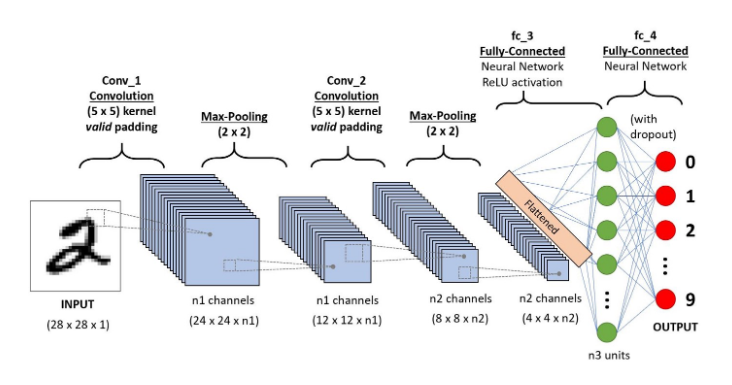
\includegraphics[scale=0.7]{images/cnn.PNG}
		\end{center}
		\caption{Rețea neurală convoluțională \newline
			\hspace{\linewidth}https://towardsdatascience.com/a-comprehensive-guide-to-convolutional-neural-networks-the-eli5-way-3bd2b1164a53}
		\label{fig:cnn}
	\end{figure}

	În Figura \ref{fig:cnn}, avem un exemplu de arhitectură de rețea convoluțională care face clasificarea unor cifre (setul de date mnist). Putem observa că măștile aplicate succesiv asupra pozelor dobândesc capabilitatea de a interpreta diferite caracteristici din cadrul acestor imagini. În final, cu ajutorul unui strat conectat, putem clasfica care cifră este expusă în poză.
    
    \clearpage
    \subsection{Rețele autoencoder}
    Un impediment întâlnit în cadrul antrenării rețelelor neurale este dat de obținerea unui set de date concludent pentru anumite testări. În domeniul abordat (procesarea audio de semnal), nu am avut posbilitatea de a găsi un număr mare de seturi de date, unele dintre ele nefiind gratis. Astfel, următorul pas în cadrul îmbogățirii setului de date a fost cel de generare sintetică a datelor, având o similaritate destul de mare cu cele originale. O metodă utilizată a fost cel al utilizării rețelelor autoencoder. Aceste rețele de tip feedforward au rolul de a învăța în mod nesupervizat datele într-o manieră codificată. Aceasta compresează datele într-un spațiu dimensional mai mic, apoi le reconstruiesc plecând de la această reprezentare. Utilizând aceste rețele asupra datelor, vom putea produce noi date (pe baza codificării învățate de aceastea), având un mic zgomot prezent (fiind o caracteristică bine venită). 
    
    \begin{figure}[H]
    	\begin{center}
    		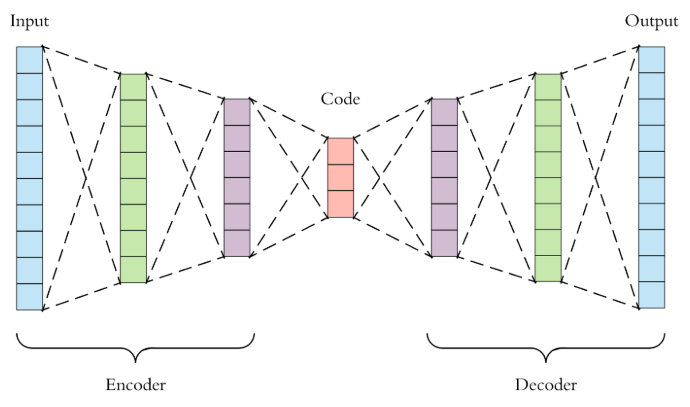
\includegraphics[width=\linewidth]{images/autoencoder.PNG}
    	\end{center}
    	\caption{Rețea autoencoder \newline
    		\hspace{\linewidth}https://towardsdatascience.com/applied-deep-learning-part-3-autoencoders-1c083af4d798}
    	\label{fig:autoencoder}
    \end{figure}
    
    În general, la fel cum se observă și în Figura \ref{fig:autoencoder}, o arhitectură de tip autoencoder este alcătuită din două subrețele:
    
    \begin{itemize}
    	\item Subrețeaua encoder, având rolul de a codifica datele de intrare în mod nesupervizat. Această subrețea va produce codul care vor reprezenta datele care vor fi propagate subrețelei decoder.
    	\item Subrețeaua decoder, care va primi numai codul din subrețeaua anterioară, va avea datoria de a produce un output veridic inputului.
    \end{itemize}

	Putem observa cum arhitecturile celor două subrețele sunt făcute în oglindă. Ansamblul celor două constituie o rețea de tip autoencoder. Pe lângă motivul utilizat în cadrul acestei licențe (generare de date), aceste rețele se mai folosesc în următoarele circumstanțe: 
	
	\begin{itemize}
		\item Detectarea anomaliilor (rețeaua se antrenează pe anumite date, iar rezultatul oferit de către funcția de cost ne poate arăta cât de diferită este data testată față de cele din setul de date, detectând o anomalie dacă această valoare de cost este mare)
		\item Reducerea zgomotului din imagini/fisiere audio (spre ex. pe baza unui input zgomots, rețeau antrenată pe setul de date curat, va putea sa reproducă pe baza inputului un ouput veridic și apropiat setului de antrenare).
	\end{itemize}
 
	În următorul capitol, vom introduce aplicația Pianify, o aplicație de transpunere a notelor muzicale, recunoaștere și separare a instrumentelor, axându-ne în principiu pe modulul de identificare muzicală.
    
    \clearpage
    \section{Aplicația Pianify}
  	Pianify este o aplicație desktop, scrisă în limbajul C++ care utilizează diverse tehnici de procesare a semnalelor cu scopul recunoașterii notelor muzicale precum și a instrumentelor de proveniență. Prezentarea aplicației se va face în două module, în care vom pune accent pe cel din urmă, fiind capitolul tratat în această lucrare. Astfel zis, modulele abordate în cadrul acestei aplicații sunt:
  	\begin{itemize}
  		\item \textbf{Modulul de "Midificare"} (Tabularizarea unei melodii într-un format ușor interpretabil de diverse programe software)
  		\item \textbf{Modulul de "Recunoaștere"} (Recunoașterea a două instrumente din melodie si separarea acestora pe track-uri diferite)
  	\end{itemize}
  	Pentru început, vom vorbi despre tehnologiile utilizate (limbaje de programe, biblioteci, medii de dezvoltare etc)  urmând mai apoi să vorbim despre rolul fiecărui modul, acceptul fiind pus pe modulul "Recunoaștere".
  	\subsection{Tehnologii}
  	Când vine vorba de programare, direcția în care se îndreaptă acest domniu este acela de a îndeplini o anumită funcționalitate cât mai specifică. Putem să ne referim la acest proces ca fiind actul de a scrie cod, care trebuie să indeplinească întotdeauna așteptările emise în faza de proiecție, testare sau design. În funcție de cerințele aplicației și aptitudinile programatorului, trebuie să alegem dintr-o gamă largă de limbaje de programare, dintre care le putem enumera pe următoarele: C, C++, Java, Python etc.
  	
  	\subsubsection{Ierarhizarea limbajelor de programare}
  	Diferite limbaje de programare oferă diferite metode de dezvoltare, făcându-se referire ca fiind paradigme ale programării. În funcție de cerințele aplicației, criteriile impuse de către companie (dacă este cazul), programatorul este nevoit să facă o alegere, care în general, nu este una foarte ușoară. Cel mai probabil, un individ care este experimentat în Python va opta în a folosi acel limbaj față de unul în care nu are experiența necesară. Un aspect importat de care trebuie ținut cont în cadrul acestei etape o reprezintă gama de utilizatori a acelei aplicații. Trebuie să ne gândim în ce domeniu se va încadra aplicația dezvoltată (diverstisment, gestionare etc) și ce sisteme de opera vor putea utiliza această unealtă. Aceste decizii vor influența în mod colosal alegerea limbajului de programare. Trebuie notat că aceste limbaje se clasifică în 3 categorii \cite{lang_clas}: 
  	\begin{itemize}
  		\item Limbaje de nivel jos; Sunt acele limbaje care sunt apropiate la nivel de cod mașină, neavând niciun fel de abstractizare sau foarte puțină față de hardware (deoarece lucrează direct cu registrii și memoria calculatorului). De menționat faptul că din moment ce instrucțiunile scrise la acest nivel lucrează direct cu hardware-ul, codul scris este dependent de sistem și nu poate fi portat (ex. Assembly).
  		\item Limbaje de nivel mediu; Aceste limbaje încep să aibă deja o abstractizare, sintaxa devenind ușor interpretabilă. Încă sunt destul de strâns legate de hardware (ex. nevoia de eliberare de memorie alocată în mod manual de către programator vs garbage collector, folosit în limbajele de nivel înalt). Putem menționa în cadrul acestei categorii limbajele C/C++.
  		\item Limbaje de nivel inalt; Aceste limbaje sunt foarte similare cu limbajul uman. Mentenanța asupra programlor scrise în limbaje de acest nivel este realizata intr-un mod facil, fiind ușor de învățat de către programatorii începători. Acestea nu comunică într-un mod direct cu hardware, ocupându-se mai degrabă pe partea de eficientizarea codului si "readability" (capacitatea de a întelege instrucțiunile într-un mod rapid). Aceastea pot fi limbaje compilate (C\#, Java) sau interpretate (Python, SQL).
  	\end{itemize}
  
  	\subsubsection{Limbajul C++}
  	Limbajul C++  este un limbaj compilat care se încadrează în categoria mid-level. Acesta a fost creat de către Bjarne Stroustrup ca o extensie a limbajului C. Apărut în jurul anului 1985, C++ a suferit multiple modificări, ajungând să ofere suport pentru programarea obiect orientată, programare generică precum și cea funcțională. 
  	
  	Fiind un limbaj compilat, codul rezultat în urma executării instrucțiunilor este unul optim și rapid (mulțumită numeroaselor optimizări făcute la nivel de compilator). Datorită acestui atribut, C++ este utilizat în numeroase domenii printre care: aplicații grafice (datorită folosirii cât mai optime a resurelor, ex: Adobe Ilustrator), sisteme de operare ( Windows 95-XP), jocuri video. În cadrul acestei aplicații, limbajul C++ este folosit ca limbaj princpial, deoarece multiple functionalități ale acestei aplicații sunt costisitioare din punct de vedere al executării lor. 
  	
  	În schimb, o serie de experimente în cadrul modului de indetificare a instrumentelor muzicale au fost îndeplinite cu ajutorului limbajului de programare Python. 
  	
  	\subsubsection{Limbajul Python}
  	La fel cum a fost menționat, Python este un limbaj de programare interpretat de nivel înalt. Creat de Guido van Rossum în anul  1991 (și utilizat cu motive interne în cadrul companiei Google), Python abordează ca valorea ușurința interpretării codului de către programatori, favorizând spațierea față de parantezele accolade. Este un limbaj care oferă suport pentru programare obiect orientată, generică precum și funcțională, venind în sprijinul programatorului cu renumitul "garbage-collector". Acesta are rolul de a elibera memoria în mod automat, de a o segmenta și de a o prealoca pentru utlizator (Python memory manager). 
  	
  	Fiind un limbaj de nivel înalt avem ca avantaje următoarele atribute: compatibilitate între sisteme (putem utiliza programale scrise in acest limbaj independet de platformă), o bibliotecă integrată foarte bogată (acest limbaj vine la pachet cu un arsenl de module care vin în sprijinul necesităților noastre), acces la multe framework-uri și unelte open-source, abilitatea de a scrie cod complex într-o manieră ușoară. Motivul utilizării acestui limbaj este dat de accesul la o multitudine de biblioteci care ne oferă suport pentru procedeele de procesare de semnal precum și construirea, antrenarea diferitelor rețele neurale.
  	
  	\subsubsection{Framework-uri și biblioteci utilizate}
  	Mai departe, vom enumera o serie de tehnologii și frameworkuri care au venit în sprijinul dezvoltării acestei aplicații. Pentru început vom discuta despre noțiunea de sistem de versionare. Un astfel de sistem are ca și caracteristici abilitatea de a ține evidența codului scris și capabilitatea de a lucra cu mai multe persoane pe aceleași fișiere. Am ales utilizarea Git-ului, care este un sistem de versionare distribuit. Din punct de vedere al mediului de lucru, am ale Visual Studio, fiind un IDE puternic care ofeă multiple funcționalități, venind în sprijinul programatorului.
  	
  	Aplicația Pianify se poate folosi în două forme: prin utilizarea liniei de comandă și prin comunicarea cu o interfață grafică construită cu ajutorul\textbf{ framworkului Qt}. Acesta este un framework open-source, care ne ajuta la dezvoltarea aplicațiilor pentru desktop, embedded sau mobile, oferind suport cross-platform (Windows, Linux, Androi, iOS etc). În general sunt două moduri de a utiliza acest framework: 
  	 	
  	\begin{itemize}
  		\item Utilizand modulul Widget;
  		\item Utilizand modulul Quick.
  	\end{itemize}
  
  	Pentru procesarea de semnal sub limbajul C++, am utilizat biblioteca\textbf{ Aquila}, o bibliotecă open source și cross-platform scrisă în standardul C++11 de către Zbigniew Siciarz. Am ales utilizarea acestui pachet de DSP datorită următorelor caracteristici:
  	
  	\begin{itemize}
  		\item compatibilitatea lucrului cu tipuri diferie de semnal (ex. generatoare, text/binar/wav);
  		\item capacitatea de a executa tehnici precum filtrarea și segmentare asupra semnalelor;
  		\item abilitatea de a manevra diferite metode de procesare (FFT, STFT, DCT)
  		\item extragerea unor serii de coeficienți (MFCC, HFCC)
  	\end{itemize}
  
  	Obiectivul primului modul, "Midificare", este acela de a transpune o melodie, de preferat un cântec de pian, într-un format care este interpretabil de cat mai multe aplicații software existente specializate pe redarea fișierelor audio. După o seria de cercetări, s-a ajuns la rezultatul că un format optim este reprezentat de midi (format ce va fi explicat în capitolul ce urmează). Pentru îndeplinirea acestui obiectiv, am utilizat biblioteca Midifile, care ne permite să citim/scriem fițiere standard în format midi.
  
  	În al doilea modul, am decis antrenarea unei rețele neurale. Acest lucru a fost îndeplinit cu ajutorul limbajului Python datorită pachetelor disponibile în cadrul acestui limbaj. Comunicarea dintre rețeaua neurală (utilizată în Python) și interfața grafică (scrisă în C++) a fost facută cu ajutorul unei conexiuni de tip server-client (TCP/UDP), folosindu-ne de modulul ASIO din cadrul bibliotecii BOOST. Nu este singurul motiv al folosirii acestei biblioteci, ea find utilizată cu scop general în cadul aplicației. Pentru submodulul reprezantat de separarea instrumentelor dintr-o melodie, acest tip de conexiune nu este foarte facilă datorită pierderilor de pachete în timpul comunicării. În acest caz, am decis utilizarea bibliotecii Tiny-DNN, o bliblioteca specializată în crearea rețelelor neurale, scrisă în C++, care ne oferă posibilatea de a construi un model de învățare automat în funcție de necesitățile noastre. 
  	
  	În final, pentru a putea face o îmbinare între aceste tehnologii, am ales utilizarea uneltei CMake, o unealta open-source, cross-platform care permite folosirea framework-urilor menționate în acest capitol într-un mod organizat. CMake ne permite să construim aplicații independete de platformă, să separăm fișierele executabile de cele binare și sa realizăm împărțirea codului în module cu scopul construirii unei ierarhii. 
  	
  	Aceste unelte software discutate mai sus reprezintă pilonii de bază al aplicației Pianify, care fac posibilă utilizarea celor două funcționalități primare. Tehnicile de preprocesare de semnal ne ajută să identificăm acele frecvențe principale din fiecare fereastră, urmând mai apoi să "midificăm" melodia. 
  	
  	În capitolul următor, vom începe modulul de identificare a notelor, explicând arhitectura aplicației precum și aplicabilitatea conceptelor de procesare digitală de semnal și învățare automată explicate până acum.
  	
  	\clearpage	
  	\subsection{Modulul "Midificare"}
  	\subsubsection{Introducere}
   	Primul modul presupune identificarea notelor muzicale dintr-o melodie și transpunerea lor într-o partitură ușor interpretabilă de diferite aplicații software (ex. Synthesia, Audacity). După cum am explicat în secțiunea de procesare de semnal, un fișier audio reprezintă un semnal în care vibrațiile sunt propagate prin intermediul aerului. Știind acest lucru, putem asocia destul de simplu o frecvență unei note muzicale. Vom utiliza o asociere standard care se folosește la nivelul tabular (utilizat și de către pian) între note și frecvențele emise de către acestea. În tabelul \ref{tab:freq_to_tab}, putem observa câteva note asociate unor frecvențe.    
   	
   	
   \begin{table}[htbp]
   \centering
   \begin{tabular}{ |c|c|c| } 
   		\hline
   		Numărul cheii & Notă pian & Frecvența emisă (Hz) \\
   		\hline
   		49 & A4 & 440.00 \\ 
   		\hline
   		40 & C4 & 261.62  \\
   		\hline
   		37 & A3 & 220.00  \\
   		\hline
   		20 & E2 & 82.40  \\
   		\hline
   \end{tabular}	
   \caption{Asociere între frecvențe și notele muzicale}
   \label{tab:freq_to_tab}
   \end{table}
	
	\subsubsection{Arhitectura}
	Prima iterație experimentală în cadrul dezvoltării acestui modul a fost reprezentat de înțelegerea și utilizarea transformatei Fourier și ale derivațiilor acesteia. Am început prin plotarea semnalelor acustice într-un sistem de coordonate XOY în care axa X este reprezentată de timp (în secunde) iar axa Y este amplitudinea. 
	
	\begin{figure}[H]
		\begin{center}
			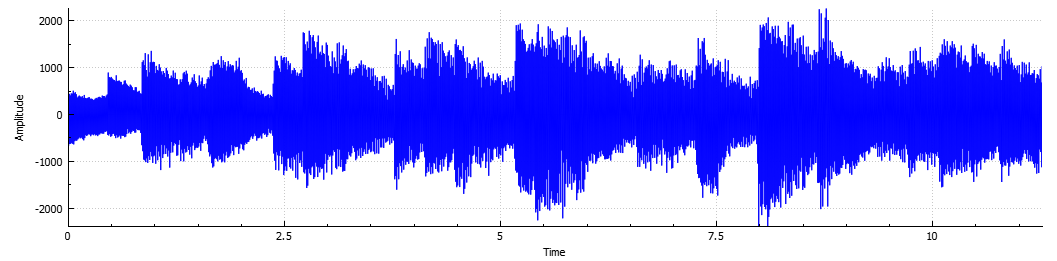
\includegraphics[width=\linewidth]{images/pianify_signal_plot.PNG}
		\end{center}
		\caption{Plotarea semnalului în Pianify}
		\label{fig:pianify_signal_plot}
	\end{figure}
    
    Utilizând suportul grafic oferit de framework-ul Qt, am reușit să plotăm un astfel de semnal și să înțelegem influența majoră a ratei de eșantionare în cadrul procesării semnalelor. În Figura \ref{fig:pianify_signal_plot}, este plotată o melodie cântată la pian, în care putem observa un pattern, o anvelopă reprezentată de fiecare apăsare a unei clape de pian. O analiză mai amănuntă a fost posibilă utilizând aplicația Audacity, foarte folositoare în cadrul întelegerii armonicelor (frecvențe care pot fi de 2,3,4 etc ori mai mari față de frecvența analizată, însă având amplitudinea în descreștere) și al evăluarii rezultatelor obținute utilizând tranformata Fourier scrisă de către noi.
    
    Înțelegând câteva detalii legate despre semnalul acustic primit ca dată de intrare, proiectul a avut ca start implemetarea transformatei Fourier. Am ales să implementăm acest procedeu pentru a avea o mai bună înțelegere a acestei unelte puternice. 
    
    După îndeplinirea acestei sarcini, s-au comparat rezultatele obținute prin utilizarea implementării noastre, cu alte aplicații software specializate pe aceste tipuri de analiză. Surprinderea noastră a fost de avea rezultate asemănătoare (frecvențe identificate în același loc în ambele aplicații). Însă, pentru semnale acustice mari din punct de vedere al timpului, cum ar melodii care pot depăși mai mult de câteva secunde, acest procedeu devine destul de costisitor, ajungând la înghețarea aplicației și terminarea ei în mod brusc. 
    
    Acest eveniment nu a fost un impediment major, deoarece după investigații amănunțite, am descoperit transformata Fourier pe termen scurt, o tehnică asemănătoare cu cea clasică, care însă fragmentează semnalul în bucați de dimensiuni egale de putere a lui 2. Această tehnică este prezentă și în biblioteca Aquila, însa asemănător cazului anterior, am decis implementarea ei pentru o mai bună înțelegere. 
    
    Având aceste tehnici, am trecut la următorul pas, cel al identificării notelor muzicale. Un impediment întâlnit în cadrul acestui pas a fost dat de necunoașterea apriori a numărului de frecvențe maxime pe care trebuie să le identificăm în ferestre. Cu alte cuvinte, nu stiam câte note vor apărea pe fiecare secvență muzicală. Acest lucru ne-a constrâns în utilizarea unui hiperparametru \textbf{k} (numărul maxim de frecvențe identificate pe o fereastră). Astfel zis, devine datoria utilizatorului de a găsi acel k potrivit în funcție de piesa aleasă pentru transpunerea ei în format midi.
    
    În funcție de rata de eșantionare, durata unei ferestre obținută în urma aplicării tranformatei Fourier pe termen scurt și numărul de secunde din melodie, am putut găsi durata unei astfel de ferestre. Acest lucru este de dorit deoarece prin intermediul acestei informații, putem cunoaște durata unei astfel de note muzicale identificată. Alte experimente făcute în cadrul acestei etape au fost reprezentate de utilizarea unor fișiere wav care conțin doar o notă muzicală reprezentată de clapa A4 (având frecvența de 440 Hz) care a fost menținută pe diferite perioade de timp. Algoritmul a fost capabil să recunoască această continuitate a notei. Însă în aceste experimente, am întâlnit un alt impediment reprezentat de armonice.
    
    Pe scurt, o armonică este un val de vibrații care este adăugat peste vibrația care a produs-o. Spre exemplu, ne putem referi la un violonist. Când acesta cântă la vioară prin intermediul arcușului, corzile încep să vibreze într-un mod foarte rapid. Vibrațiile fac ca mediul de propagare (aerul) să vibreze și să transmită aceste unde sonore urechilor noastre, urmând mai apoi să îl identificăm. Dacă nota este absolut pură din punct de vedere al frecvenței (ceea ce se întâmplă rar), această undă sonoră s-ar transmite într-un mod sinusoidal provocând apariția unei singure frecvențe, aceea find nota de bază. Dar, în schimb, pe lângă această notă, alte multiple frecvențe sunt produse. 
    
    Aceste frecvențe minore care apar pe lângă nota principală sunt acele care ne spun că nota aparține unei vioare și nu unui clarinet. Putem deduce din ce am discutat până acum referitor la armonice că sunt defapt un lucru bun. În cadrul identificării notelor, acestea sunt înșelătoare, deoarece ne pun la încercare abilitatea de a recunoaște notele principale din fiecare fereastra muzicală. Sunt șanse ca nota identificată în fereastra \textbf{i} să producă o armonică în fereastra \textbf{i + 1}. Acesta poate masca notele care defapt sunt acele note principale pe care dorim să le identificăm. Pentru a evita luarea lor în evidență, cel mai util mod este acela de a calcula dacă nota muzicalâă este o armonică sau nu.
    
    Avand frecvențele, duratele lor și ferestrele în care apar, următorul pas pe care l-am luat în considerare a fost cel al transformării frecvențelor găsite la cele standard. Este puțin probabil ca atunci când facem analiza unui semnal acustic, să identificăm o frecvență care este fix 440 Hz spre exemplu. Pentru acest caz am calculat distanța medie a frecvenței identificată la fiecare din cele 108 note interpretabile de un pian. Standardul acestor note muzicale deja presupune tranformările din frecvență la note și invers. Pentru transformarea unei note muzicale în frecvență putem utiliza:
    
    \begin{equation}
  		\label{note_to_freq}
    	f(n)= 2^{\frac{n-49}{12}}*440
    \end{equation}
    
    unde n reprezintă numărul cheii pe care dorim să o tranformăm în frecvența corespunzătoare, iar f, rezultatul în Hz. Pentru procedeul invers asociat formulei \ref{note_to_freq} putem utiliza:
    
    \begin{equation}
    \label{freq_to_note}
    n = 12 * log(\dfrac{f}{440}) + 49
    \end{equation}

    Frecvențele mapate pe ferestre nu au fost îndeajuns pentru a putea transpune piesa în partitură, sub contextul fisierului de format midi. În cadrul acestui format, unitate de măsură pentru timp nu este reprezentată de secunde, ci de tics (o oarecare reprezentare a conceptului de bătăi pe secunde). Pentru a întelege acest mecanism, a trebuit să experimentez lucrul cu biblioteca MidiFile pentru a putea dobândi experiența necesară creării acestor tipuri de fișiere. 
    
    MIDI (acronim pentru Musical Instrument Digital Interface) reprezintă un standard care descrie un protocol de comunicare, o interfață digitală și conectori electronici care conectează o gamă largă de instrumente electronice, calculatoare și dispozitive audio folosite pentru redare, editare și înregistrare. 
    
    Specificațiile acestui tip de fișier au luat naștere printr-o publicație făcaută de Dave Smith si Chet Wood, anul 1981 în cadrul conferinței societății de ingineri audio New York. Un singur fișier midi poate avea până la 16 canale, unde fiecare canal poate reprezenta un instrument (aceste instrumente pot fi diferite de exemplu). MIDI are integrat un sistem care specifică o multitudine de instrucțiuni referitoare la muzică, cum ar fi: notația muzicală a notelor standard, pitch-ul, velocity (care se face referire adesea ca fiind loudness), panning (efectul de stereo), tempo-ul.
    
    Printe avantajele acestui tip de format, le putem menționa pe următoarele:
    \begin{itemize}
    	\item Fișierele nu ocupă mult spațiu;
    	\item Manipulare și modificare ușoară a configurațiilor;
    	\item Gamă largă de instrumente, sintetizatoare sau sunete digitale din care putem alege.
    \end{itemize} 
        
    Odată dobândită această aptitudine, împreună cu rezultatul obținut în pasul anterior (frecvențele mapate pe ferestrele corespunzătoare), am reușit transpunerea melodiei prin identificarea notelor. Instrumentele muzicale de redare a rezultatului se pot modifica într-un mod foarte ușor, printr-o schimbare a unei variabile care reprezintă instrumentul pe care dorim să îl auzim in fișierul midi. Acest fapt ne face trimitere la maniera ușoară în care putem face trecerea la modulul de recunoaștere a instrumentelor.
    
    \clearpage
    \subsubsection{Detalii de implementare}
    Considerând toate conceptele discutate anterior, putem defini următorul algoritm pentru producerea rezultatului dorit:
    
    \begin{itemize}
    	\item Aplicarea tranformatei Fourier pe melodia primită ca dată de intrare; În cadrul aplicației, utilizatorul va fi nevoit să aleagă una din cele trei metode de a procesa melodia în domeniul frecvențelor:
    	\begin{itemize}
    		\item Fast Fourier Transform
    		\item Short Time Fourier Transform
    		\item Aquila Short Time Fourier Transform
    	\end{itemize}
    	În functie de decizia aleasă de către utilizator, partitura va fi creată în fișierul midi utilizând algoritmul selectat. Diferențele majore în algoritmii enumerați sunt date de acuratețea identificării notelor precum și timpul necesar efectuării lor.
    	\item Extragerea frecvențelor predominente în funcție de hiperparametrul \textbf{k} ales de către utilizator sau prin identificarea singură a acesteia; Acesta nu poate fi mai mare sau egal cu zero. În cazul în care nu dorim să alegem acel hiperparametru sau nu știm ce valaore ar fi potrivită, există și opțiunea "Variable Extraction". Aceasta presupune extragerea într-un mod variabil a frecventelor, de la fereastră la fereastră.
    	\item Maparea frecvențelor și a ferestrelor în care apar acestea; Fiecare notă idetificată în ferestrele analizate va fi asociată ferestrei în care a fost gasită precum și numărul de ferestre consecutive în care apare.
    	\item Sortarea lor în funcție de apariție și durată din punct de vedere al secundelor; Dupa maparea făcută la pasul anterior este necesar să sortăm notele idenficate pentru a putea face transpunerea în mod corect în fișier midi. 
    	\item Scrierea lor într-un fișier midi. Se va scrie un fișier de format midi care va conține piesa transpusă într-o partitură. Acesta va putea fi alcătuit mai multe track-uri, trăsătură folosită în cadrul modulului de separare a instrumentelor, pentru a putea scrie fiecare instrument identificat și separat, pe un track diferit.
    \end{itemize}


	Pentru a putea reda rezultatul obtinut, ne vom folosi de o aplicație third party, Synthesia. Această aplicație este un emulator de pian, dezvoltată pentru mai multe platforme (Windows, Mac OS si Android) care permite utilizatorilor să utilizeze o orgă virtuală MIDI pe post de clapele pianului. Alegerea acestei aplicații este motivată de vizualizarea rezultatului obținut, datorită interfeței grafice (asemănător jocului Guitar Hero) deoarece oferă suport utilizatorului să cânte partitura și să vizualizeze durata notelor, precum și instrumentul utilizat.   
	
	\begin{figure}[H]
		\begin{center}
			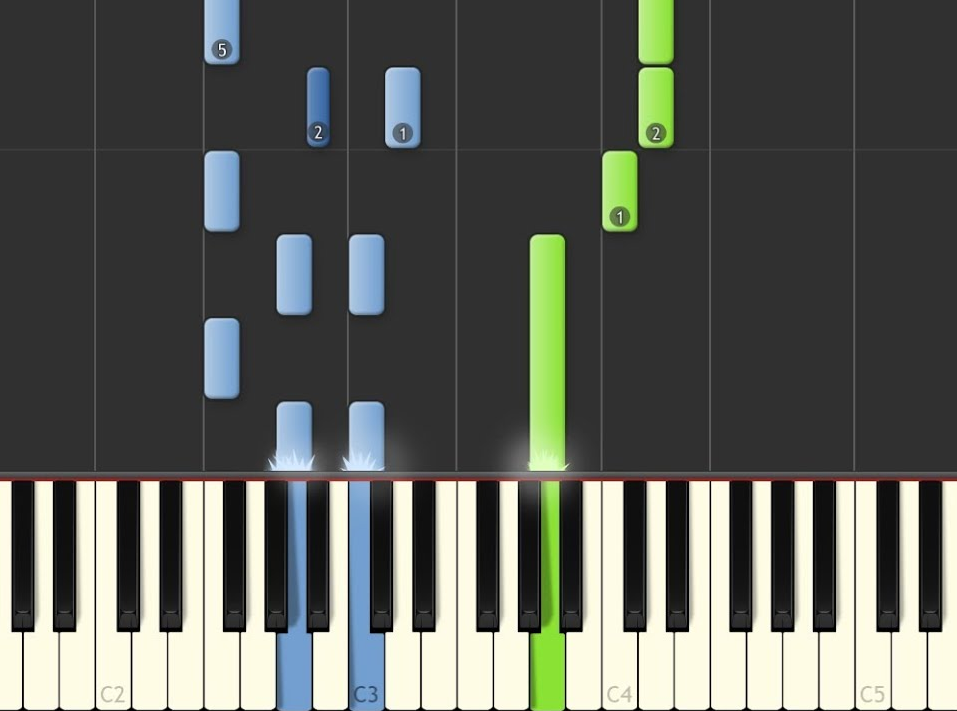
\includegraphics[scale=0.4]{images/synhesia.PNG}
		\end{center}
		\caption{Aplicația Synthesia}
		\label{fig:synthesia}
	\end{figure}

	Atunci când redăm un fișier midi în această aplicație, vom fi întâmpinați de o interfață asemănătoare Figurii \ref{fig:synthesia}. Putem observa cum notele "cad" iar în momentul în care acestea ating clapele pianului, utilizatorul este obligat să apese clapa corespunzătoare (adnotată cu notele standard). Fiecare instrument este reprezentat de o culoare (în cazul nostru, albastru și verde). Cu cât este mai lungă nota, cu atât utilizatorul va fi nevoit să mențină tasta corespunzătoare apăsată.
	
   \clearpage
   \subsection{Modulul "Recunoaștere"}
   În cadrul acestui modul, obiectivul principal a fost acela de a identifica instrumentele principale din piesa analizată precum și de ale separa pe track-uri diferite. În cadrul acestui modul, modelele de învățare automată ne-au fost de folos, deoarece acești algoritmi sunt capabili să învețe diferite trăsături pe baza unui set de antrenare. 
   
   Pentru cereințele acestui modul, un impediment major pe care l-am întâmpinat a fost cel al găsirii unui set de date optim. Dar ce reprezintă termenul optim în contextul nostru? Putem spune că un astfel de set de date care să îndeplinească minimul așteptărilor noastre ar fi acela care să conțină date din aceeași categorie a problemei pe care încercăm să o rezolvăm. 
   
   În cazul acestui modul, avem nevoie de date care să reprezinte sunete de instrumente. Instrumentele pe care dorim să le identificăm sunt pian și trompetă. Aceste instrumente au fost alese datorită diferenței date de anvelopele lor muzicale. Înca un aspect necesar pe care l-am urmărit în alegerea setului de date a fost rezoluția ratei de eșantionare. Cu cât avem o rată de eșantionare mai mare, cu atât sunetele din cadrul setului de date vor fi de o calitate mai mare din punct de vedere sonor. Fiind o problemă de clasificare, dorim ca datele de antrenare să aibă clasele atașate în mod corect. Urmărind aceste criterii, am ales setul de date IRMAS.
   
   
   \subsubsection{Setul de date IRMAS} 
   IRMAS \cite{irmas} este un set date construit pentru antrenarea și testarea algortimilor de învățare automată specializați pe identificare instrumentelor muzicale predominante. Instrumetele care aparțin acestui set de date sunt următoarele: violoncel, clarinet, flaut, chitară acustică, chiatară electrică, orgă, pian, saxofon, trompetă, vioară și melodii cântate de către artiști. Acest set de date este derivat dintr-un set de date construit de către Ferdinand Fuhmann în cadrul lucrării sale de doctorat, modificările constând în formatul stereo abordat.
   
   Setul de date IRMAS este împărțit în set de antrenare și set de testare:
   \begin{itemize}
   	\item Setul de antrenare este format din 6705 fișiere audio wav având bit depth-ul de 16 biți, stereo, înregsitrate la o rată de eșantionare de 44.1 KHz. Fiecare fișier audio este alcătuit din 3 secunde, aparținând a peste 2000 de înregistrări distincte. Adnotările instrumentelor predominante sunt reprezentate de 3 caractere: cel (violoncel), cla (clarinet), flu (flaut), gac (chitară acustică), gel (chitară electrică), org (orgă), pia (pian), sax, (saxofon), tru (trompetă), vio (vioară) și voi (voce). Acest set de date este alcătuit din melodii care aparțin mai multor genuri muzicale apărute în decursul ultimelor decenii. Aceste melodii din setul de date sunt variate din punct de vedere al instrumentelor utilizate, al stilulio abordat de către muzicieni, al acordărilor precum și al echipamentului de înregistrare din cadrul firmei de producție. În plus, în setul de date IRMAS se încearcă o maximizare a distribuției genurilor muzicale cu scopul de preveni algoritmii de învățare automată să extragă informații legate de genul muzical. Chiar dacă apar și instrumente secundare în cadrul unui fișier audio, acestea nu ar trebui să interfereze într-un mod negativ asupra modelelor de machine learning. Ba din contră, adăugarea de un astfel de zgomot dezvoltă alte capabilități interesante ale acestor algorimti de a se adapta.
   	\item Setul de testare este alcătuit din 2874 fișiere audio wav având bit depth-ul de 16 biți, stereo, înregistrate la o rată de eșantionare de 44.1 KHz. Din punct de vedere al adnotărilor, în aceste fișiere nu este specificat instrumentul/instrumentele, aceastea nefăcând parte din setul de antrenare.
   \end{itemize}
	
	Din cadrul acestui set de date, s-a ales recunoașterea a două intrumente muzicale, acelea fiind pian și trompetă. Motivul din spatele acestei alegeri este susținută de anvelopa acustică a celor două sunete, fiecare instrument având un timbru diferit, rezultând într-o recunoaștere mai sigură a sunetului.
	
	Un impediment întâlnit în cadrul antrenării algoritmilor de învățare automată a fost cel al numărului mic de date. În general, pentru a avea un model de învățare stabil, este nevoie de un număr cat mai mare de date, pentru o antrenare cat mai flexibilă și fiabilă. După cum este menționat și în descrierea setului de date IRMAS, acesta este destul de mic. Pentru acest neajuns, am decis utilizarea rețelelor autoencoder cu scopul augmentării numărului de date pentru învățare. Aceste rețele au avut scopul de a învăța o codificare eficientă a datelor, urmând mai apoi de a decodifica aceste sunete. Rezultatul este foarte similar cu datele utilizate deja, diferența fiind în adăugarea unui mic zgomot apărat în urma decodificării, care nu ridică niciun fel de problemă.
	  
   \subsubsection{Preprocesarea datelor și antrenarea rețelelor} 
   După cum este menționat în setul de date IRMAS, aceste sunete au o durată de aproximativ 3 secunde, la o rată de eșantionare de 44.1 KHz. Putem deduce, că un astfel de fișier audio wav va conține o secvență de 132300 de numere definite în domeniul timpului. Primul pas spre prepocesarea datelor a fost acela de a alege o metodă suficient de optimă care ne oferă rezultatele dorite. Folosirea transformatei Fourier și a derivatelor ei nu reprezintă o metodă valabilă deoarece principalul motiv al acestui modul este acela de recunoaștere a instrumentelor. Transformata Fourier ne oferă doar informații privind frecvențele predominante din cadrul fisierului audio precum și ferestrele în care apar, dar nici cum o relație între instrumentul care a produs acest sunet. În acest scop, vom utiliza tehnica de preprocesare MFC pentru a obține informațiile necesare.
   
   La fel cum este menționat și în cadrul capitolului "Coeficietenții Mel-frequency cepstral", acești coeficienți ne oferă informații strict referitoare la modul în care instrumentul sună (timbrul muzical). În cadrul preprocesării, au fost utilizate doua moduri de reprezentare a datelor, specifice celor două probleme abordate în cadrul acestui modul: recunoașterea instrumentelor muzicale și separarea instrumentelor muzicale pe o partitură reprezentată de un fișier MIDI. Vom prezenta cele două metode (ambele având rădăcini în tehnica MFC) precum și antrenarea rețelelor: 
   
   \begin{itemize}
   	\item Preprocesare datelor pentru rețeaua convoluțională, folosită cu scopul recunoașterii concentrației celor două instrumente muzicale dintr-o melodie. Datele au fost preprocesate în felul următor:
   		\begin{itemize}
   			\item Fișierele de intrare având o durată de circa 3 secunde (44100 de date) au fost segmentate în 3 fișiere audio, fiecare având o secunda durată (deci 44100 de date);
   			\item S-a aplicat transformarea în coeficienți MFC;
   			\item Fiecare din cele 3 segmente obținute în urma aplicării MFC au fost redimensionate în poze de dimensiunea 66x66. Această dimensiune s-a ales cu scopul de a reține cât mai mulți coeficienți MFC.
   		\end{itemize}
   	
   	În cadrul antrenării acestei rețele, am ales utilizarea pachetului Keras din cadrul limbajului Python datorită modului de utilizare foarte prietenos cu utilizatorul. Rețeaua a fost alcătuită din:
   		\begin{itemize}
   			\item Un strat convoluțional 2d, având un număr de 32 de filtre de dimensiune 3x3, cu funcția de activare 'relu';
   			\item Un strat de max pooling, având dimensiunea de 2x2;
   			\item Un strat convoluțional 2d, având un număr de 64 de filtre de dimensiune 3x3, cu funcția de activare 'relu';
   			\item Un strat dropout, folosit cu scopul tăierii conexiunilor între neuroni. Acest lucru face ca rețeaua să învețe alte metode de a propaga informația în rețea;
   			\item Un strat dense cu 128 de neuroni, folosit cu rolul pregătirii pentru clasificare;
   			\item Un strat dense cu 2 neuroni, care reprezintă numărul de clase pe care dorim sa le clasificăm. Funcția de activare în acest caz devine 'softmax'.
   		\end{itemize} 
   	Comunicarea între interfața grafică construită în C++ și rețeaua antrenată în Python se face prin intermediul socket-elor (comunicare de tip TCP), cu ajutorul modului ASIO din Boost. Această comunicare nu este de încredere, uneori fiind șanse ca pachetele să se piardă în timpul comunicării.
   	
   	\item Preprocesare datelor pentru rețeaua perceptron multistrat, folosită cu scopul separării celor două instrumente dintr-o melodiei și a transpunerii lor în fișier MIDI pe canale separate. Datele au fost preprocesate în felul următor: 
	   \begin{itemize}
	   		\item Fișierele audio de intrare au fost convertite în coeficienți MFC;
	   		\item Calcularea mediei a coefiecienților din fiecare fereastră rezultată în urma transformării;
	   		\item Păstrearea a unui număr de 40 de coeficienți.
	   \end{itemize}
   Antrenarea rețelei s-a efectuat cu ajutorul bibliotecii Tiny DNN, în limbajul C++, pentru a avea un răspuns prompt la clasificare. Această rețea a fost alcatuită din două straturi, pe ultimul strat fiind functia de 'softmax' pentru clasificare. Numărul de neuroni de pe fiecare start a fost ales empiric în urma unor suite de teste.
\end{itemize}
   \subsubsection{Ghid de utilizare} 
   În acest capitol vom descrie ghidul de utilizare al modulului de "Recunoaștere" precum și informații referitoare la algoritmii utilizați.
   În Figura \ref{fig:pianify_mainwindow}, suntem întâmpinați de meniul principal al aplicației. Fiecare buton este corespunzator celor două module mentionațe.
   
   \begin{figure}[H]
   		\begin{center}
   		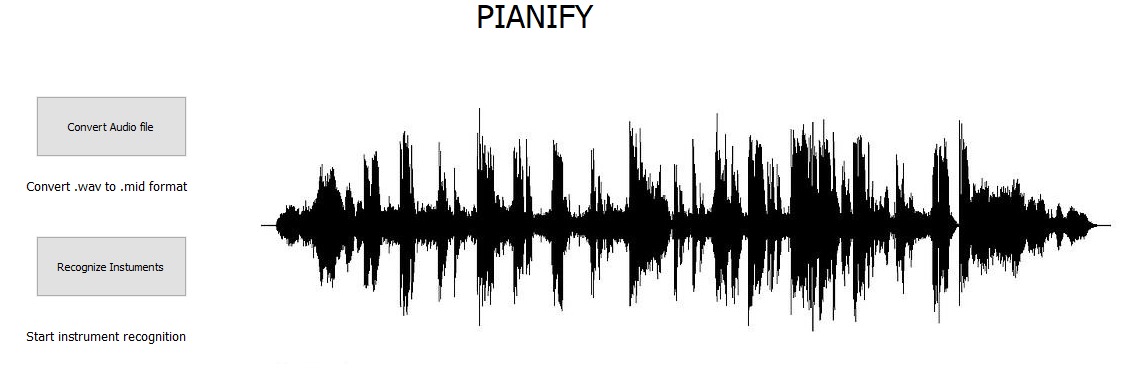
\includegraphics[scale=0.4]{images/pianify_mainwindow.PNG}
   		\end{center}
   		\caption{Aplicația Pianify - Ecranul principal }
   		\label{fig:pianify_mainwindow}
   \end{figure}
   
  În cadrul modului de "Recunoaștere", putem observa Figura \ref{fig:pianify_recognizeview}. 
   
   \begin{figure}[H]
   		\begin{center}
   		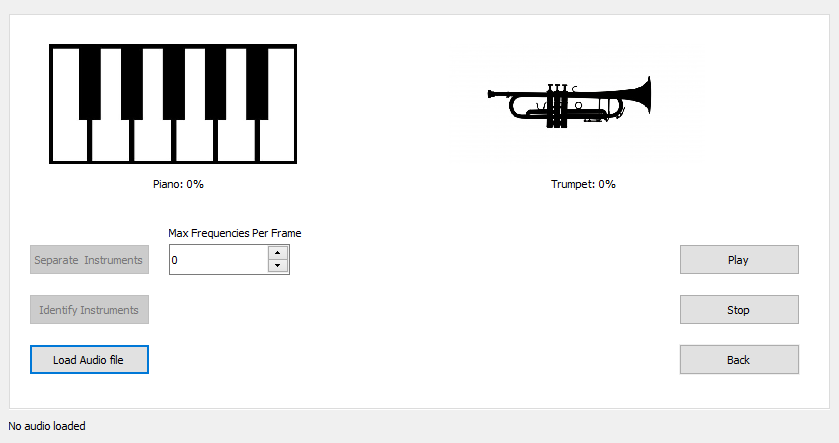
\includegraphics[scale=0.4]{images/pianify_recognizeviewPNG.PNG}
   		\end{center}
   		\caption{Aplicația Pianify - Recunoaștere}
   		\label{fig:pianify_recognizeview}
   \end{figure}
	
	Pentru început, vom detalia informații despre cele două instrumente afișate în această fereastră. Ele reprezintă principalele instrumente muzicale care pot fi identificate în urma rulării algoritmilor specifici.  Numărul antecedent simbolului \% reprezintă concentrația de instrument din piesa încărcată. Încarcarea unei melodii de tip wav se face într-un mod simplu. Apăsând butonul "Load Audio file", vom fi întâmpinați de un dialog de selectare, care filtrează în mod automat doar fisiere cu extensia .wav. 
	
	În urma încărcării unui astfel de fișier, în cadrul procesului de încărcare se va face o medie a canalelor (în cazul celor stereo). Pe scurt, se va aduce în format mono.  Butoanele din partea dreaptă a ferestrei sunt utilitare. Le putem folosi dacă dorim să ascultăm melodia încărcată (daca este prezentă), să oprim melodia dacă nu mai dorim sa o redăm sau să ne întoarcem la ecranul principal. Butoanele rămase sunt cele care descriu cele două probleme abordate în cadrul acestui modul: recunoașterea instrumentelor și separarea instrumentelor într-un format MIDI.
	
	Apăsând butonul "Identify Instruments" vom lansa în execuție algoritmul care ne va spune concetrația celor două instrumente din melodia încărcată. Primul pas este cel al fragmentării melodiei în ferestre de durată a 3 secunde. Se va utiliza tehnica de segmentare windowing (intercalare) pentru a obține o rezoluție cât mai bună a datelor. Un alt beneficiu al utilizării acestei tehnici este sugerată de folosirea numărului de date în număr cât mai mare cu putință. 
	
	Fiecare fereastră la rândul ei va fi segmentată într-un număr de sample-uri care vor fi transmise printr-o conexiune bazată pe sockete, scriptului scris in Python. Fiecare secundă va fi împărțită în 20 de segmente (știind că rata de eșantionare este de 44100 de date, vom trimite circa 2205 date per segment) ce vor fi transmise scriptului python. În interiorul scriptului, atunci când s-a atins numărul de sample-uri care reprezintă 3 secunde de sunet (44100 * 3), se va trece la pasul de preprocesare, pentru a aranja aceste date într-o formă agreată de clasificatorul antrenat. Prin preprocesare, mă refer ca se vor calcula coeficienții MFC, urmând apoi aranjarea lor într-o formă asemănătoare cu rezoluția unei poze pătratice (66 x 66). 
	
	Având datele preprocesate într-o formă validă, se va putea face o predicție pentru a determina proveniența sunetului. Reteaua CNN va face această predicție, urmând mai apoi să transmită către interfața grafică C++ categoria prezisă. În cadrul interfeței grafice, se va calcula raportul celor două instrumente urmând mai apoi să se afișeze cantitatea de apartenență a melodiei la fiecare instrument pentru a fi vizualizată de către utilizator. Având rezultatele utilizatorului, acesta va putea vizualiza raportul celor două instrumente. De notatat faptul că, atunci când melodia aleasă nu va conține niciunul din instrumentele menționate, acesta va încerca să aleagă instrumentul care are cel mai mare grad de similaritate cu cele prezente din melodie. Prin grad de similaritate, mă refer la timbrul instrumentului precum și anvelopa acustică a acestuia. 
	
	Pentru exemplificarea celei de a doua problemă abordată în cadrul acestui modul, vom utiliza butonul "Separate Instruments". Mai întâi, vom fi nevoiți să alegem o valoare numerică întreagă care reprezintă numărul maxim de frecvențe pe care dorim să le luăm în considerare în urma executării transformatei Fourier pe termen scurt. De menționat este faptul că acest număr nu poate fi mai mic sau egal cu zero. La fel cum a fost menționat și în cadrul modulului "Midificare", acestă valoare este un hiperparametru pe care utilizatorul trebuie să îl găsească în mod iterativ, rulând algorimtul de mai multe ori până se atinge acea valoare care îndeplinește criteriile cerute. 
		
	\subsubsection{Detalii de implementare}
	Având aleasă această valoare, butonul se va activa, utilizatorul putând lansa în execuție algoritmul. Pașii care vor fi executați în cadrul acestui algoritm sunt următorii:
	
	\begin{itemize}
		\item Aplicarea transformatei Fourier pe termen scurt;
		\item Extragerea notelor predominante în funcție de valoarea aleaăa la numărul maxim de frecvențe recunoscute pe fereastră;
		\item Dacă în fereastra curentă au fost identificate note, vom apela metoda de predictie a algoritmului de învățare; În funcție de clasa prezisă vom putea marca nota identificată ca sunte de pian/trompetă;
		\item Maparea notelor identicate împreună cu instrumentul identificat în funcție de fereastra în care au fost recunnoscute;
		\item Calcularea duratei fiecărei note identificate;
		\item Sortarea notelor în funcție de începutul, durata și sfârșitul lor;
		\item Exportarea unui fișier de format MIDI.
	\end{itemize}
	
	Daca vom dori redarea acestui fișier, vom fi nevoiți să folosim una din aplicațiile software menționate care pot reda astfel de fișiere. În cazul aplicației Synthesia, vom putea alege dacă dorim să redăm unul din cele două instrumente sau pe ambele. Apartenența fiecărei note la instrument se va putea identifica prin culorile diferite asignate lor.
	
   \clearpage
   \section{Monitorizarea rulmenților}  
    \subsection{Introducere}
    	Rulmenții pe bilă reprezintă o componentă esențială a tuturor mașinăriilor bazate pe echipamente rotative. Prin componente rotative, în general ne gândim la obiecte care folosesc energie cinetică pentru a mișca fluide, gaze și alte materiale (adesea utilizate în motoare, compresoare, turbine, generatoare etc).
    	
    	Datorită gamei largi de utilizare a rulmenților, orice defecțiune cauzată de aceștia reprezintă o problemă destul serioasă din punct de vedere financiar, mai ales în cazul mașinăriilor mari dar și din punct de vedere a siguranței persoanelor care sunt responsabile de controlul și întreținerea lor. Spre exemplu, în cazul unei turbine eoliene moderne, rulmenții au rolul de a putea pune în mișcare elicea, propulsată de vânt, pentru a putea produce energie regenerabilă. Fără niciun fel de întreținere predictivă (făcută în avans), defecțiunea rulmenților pot duce la oprirea întregului sistem eolian, aducând pagube financiare destul de majore companiei de întreținere responsabilă, precum și timp pierdut. 
    	
    	Cu ajutorul monitorizării stării rulmenților, putem accesa în timp real situația echipamentului. Acestă utilitate ne ajută doarece putem programa în avans lucrări de remediere sau înlocuire a rulmenților, scutind astfel companiile de costul repunerii în execuție a unui sistem blocat.
    	
    	Diferite metode tradiționale care au fost și încă sunt aplicate în cadrul monitorizării echipamentelor rotative constituie piloni de bază în analiza datelor primitie prin achiziție senzorială. Vibrațiile captate de diferiți senzori sunt mai departe preprocesați utilizând diferite tehnici de procesare de semnal, tehnici de filtrare sau metode statistice. Însă, impedimentul care răsare în aceste analize este dat de faptul că toate aceste metode sunt condiționate de interpretarea unui expert în acest domeniu, care poate da un diagnostic corect sistemului. De aici, a pornit idea utilizării învățării automate.
    	
    	Extragerea datelor cu care dorim antrenarea rețelei neurale este realizată grație metodelor de procesare de semnal (transformata Fourier împreună cu derivatele ei, coeficienții de tip MFC). Cu ajutorul acestor metode de procesare, am reușit construirea unui input valid modelelor de antrenare, acestea fiind înzestrate cu capacitatea de a recunoaște și de a învăța pattern-uri în diferite maniere.
    	
    	Punctul de plecare utilizat în cadrul acestui experiment a fost dat de lecturarea și replicarea articolul "Rolling element bearing fault diagnosis using convolutional neural network and vibration image" \cite{rolling_elemnt}. În acest articol, se experimentează clasificarea stării rulmenților, cu ajutorul rețelelor neurale convoluționale antrenate pe setul de date "Case Western Reserve University Bearing Data Center". Clasificarea care se efectuează este acea de a diferenția un rulment sănătos din punct de vedere funcțional de cei stricați (defecțiuni la cursa interioară, cursa exterioară sau bilă). În Figura \ref{fig:bearing_signals} observăm principalele categorii pe care sunt făcute clasificările precum și o reprezentare a semnalului emis de aceste stări. Se poate remarca o diferență din punct de vedere aspectual a celor patru imagini, putând deduce faptul că și o rețea poate distinge aceste semnale.
    	
    	\begin{figure}[H]
    		\begin{center}
    			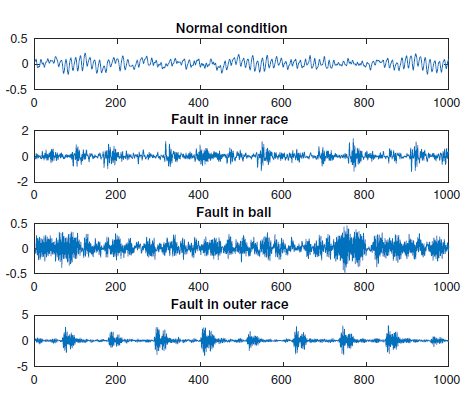
\includegraphics[scale=0.7]{images/bearing_signal.PNG}
    		\end{center}
    		\caption{Segmente de semnale ale rulmențiilor}
    		\label{fig:bearing_signals}
    	\end{figure}
    	
    	Se presupune că fiecare secvență de date (vibrațiile achiziționate cu ajutorul unui accelerometru) vor fi remodelate în imagini de dimensiunea 20x20 (Figura \ref{fig:bearing_image}), un input valid pentru rețeaua convoluțională. Fiecare 400 de sample-uri vor constitui o dată antrenabilă de rețea.
    	
    	\begin{figure}[H]
    		\begin{center}
    			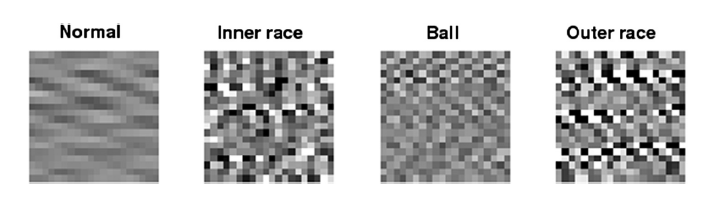
\includegraphics[scale=0.5]{images/image_bearing.PNG}
    		\end{center}
    		\caption{Semnal rulment transformat în imagine}
    		\label{fig:bearing_image}
    	\end{figure}
 	
    	\clearpage
    	\subsection{Seturi de date}
    	Setul de date principal pe care ne-am bazat în cadrul analizei distribuției frecvențelor rulmenților și a antrenării rețelei neurale este acela utilizat și în cadrul articolului menționat, Case Western Reserve University Bearing Data (CWRU). Bancul de testare (Figura \ref{fig:test_bench}) este alcătuit din următoarele componente:
    	
    	\begin{itemize}
    		\item În stânga, un motor de 2 cai putere;
    		\item În centru, un codificator;
    		\item În dreapta, un dinamometru;
    		\item Doi rulmenți fabricați de firma SKF, având mărimi diferite, amplasați de o parte și de alta a bancului de testare, pe shaftul motorului.
    	\end{itemize}
    	
    	\begin{figure}[H]
    		\begin{center}
    			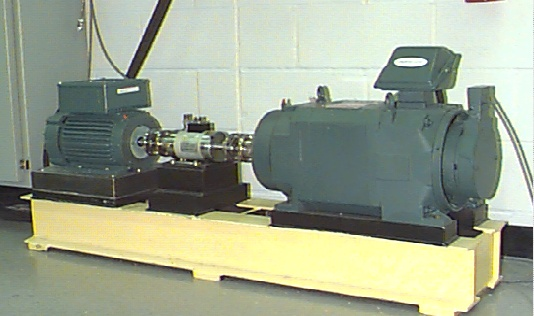
\includegraphics[scale=0.5]{images/CWRU.jpg}
    		\end{center}
    		\caption{Bancul de testare \newline
    			\hspace{\linewidth}https://csegroups.case.edu/bearingdatacenter/pages/apparatus-procedures}
    		\label{fig:test_bench}
    	\end{figure}
    
    	Pentru a putea diferenția cei doi rulmenți, vom folosi următoarea notație: rulmentul DE (Drive End) poziționat într-un capat și rulmentul FE (Fan End) poziționat de cealaltă parte. 
    	
    	Cele trei defecțiuni ale rulmenților, menționate mai sus nu au apărut din cauze naturale, precum uzura. Acestea au fost comise într-un mod artificail, prin utilizarea șocurilor electrice. Găurile provocate de acest șoc au avut următoarele diametre: 7 mm, 14 mm, 21 mm si 40 mm. 
    	
    	Rulmenții au fost mai departe puși în folosință. Utilizând diferite sarcini (0, 1, 2 și 3 cai putere pe un motor care produce viteze de la 1720 până la 1797 rotații pe minut), clasele de defecțiune (cursa interioară, cursa exterioară și bila) au fost achiziționate utilizând un senzor de tip accelerometru, la o rată de eșantionare de 12 KHz sau 48 KHz pe o perioadă de 40 de secunde. Starea de funcționare sănătoasă a rulmentului a fost înregistrată cu aceleași specificații dar pe o perioadă de 20 de secunde.
    	
    	Utilizând pachetul Matplotlib din limbajul Pyhton, s-a reușit construirea unei spectograme de tip waterfall, pentru a analiza frecvențele principale precum și continuitatea acestora pe secvențe de vibrații următoare. Am putut vedea faptul că vibrațiile predominante rămân aceleași, indiferent de fereastra în care ne aflăm, înțelegând astfel faptul că fiecare rulment are o construcție diferită și emite anumite frecvențe. În Figura \ref{fig:waterfall_bearing_healthy}, este desenată o spectogramă a unui rulment sănătos din punct de vedere funcțional. Observăm că pe parcursul secvențelor de vibratii, frecvențele rămân aproximativ în aceleași poziții.
    	
    	\begin{figure}[H]
    		\begin{center}
    			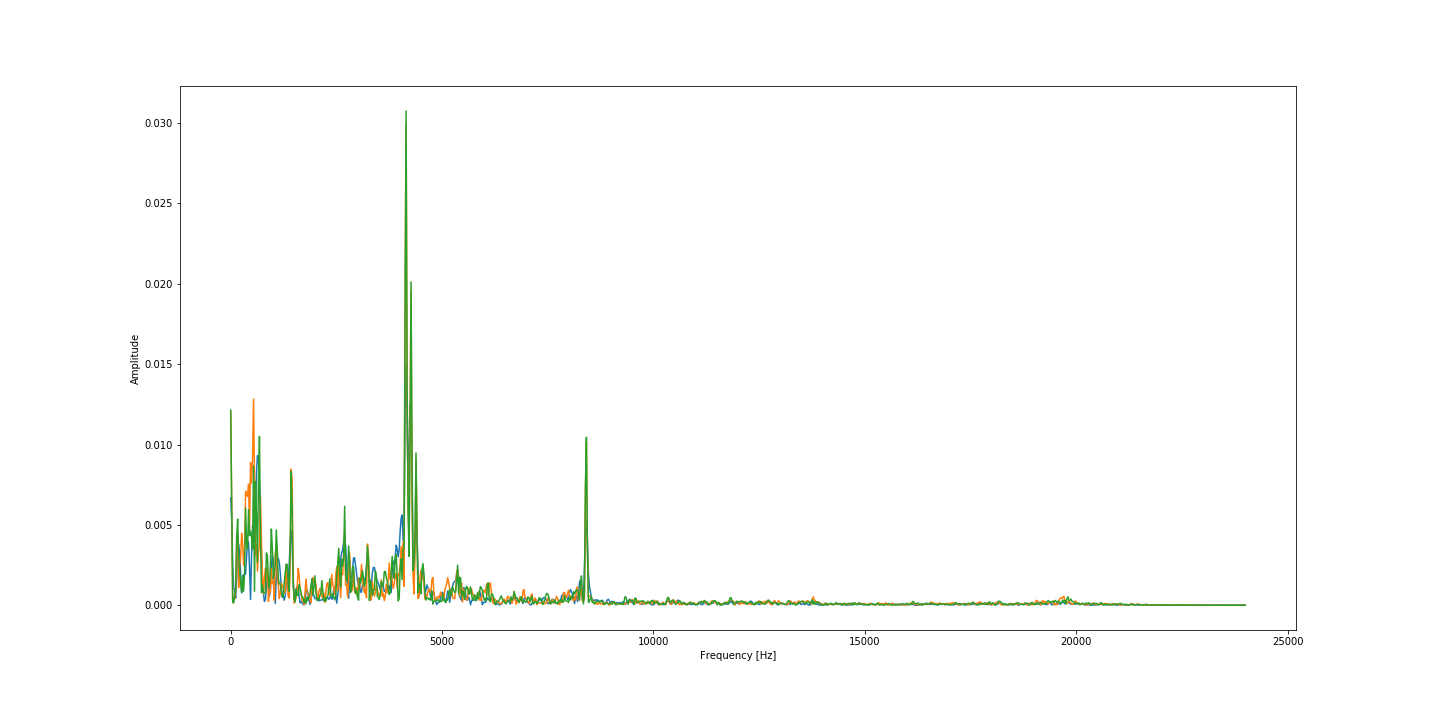
\includegraphics[scale=0.25]{images/waterfall_bearing_normal.png}
    		\end{center}
    		\caption{Spectogramă de timp waterfall pe un rulment sănătos}
    		\label{fig:waterfall_bearing_healthy}
    	\end{figure}
    	
    	Scopul principal al acestui experiment a fost acela de construi un model inteligent, capabil să recunoască stările unor rulmenți diferiți din punct de vedere al dimensiunilor și al numărului de bile. Practic, să nu depindem foarte puternic de frecvențele emise, ci mai degrabă de modul în care rulmentul sună (vibrațiile acestuia).
    	
    	Un alt set de date propus în cadrul acestor experimente și folosit mai degrabă cu scopul de a valida iterațiile experimentului a fost setul "Nasa Ames Prognostics Data Repository Bearings". În acest set de date patru rulmenți sunt expuși pe o perioadă mai lungă de tip unui motor care aplică în jur de 2000 de rotații pe minut. Diferența principală între acest set de date și CWRU este dat de maniera de defectare. În acest caz, se bazează în principiu pe uzura componentelor mecanice. 
    	
    	Modul de achiziție a datelor este următorul :
    	
    	\begin{itemize}
    		\item Pentru fiecare rulment din cei patru sunt achiziționate date utilizând un senzor de tip accelerometru;
    		\item Pe o perioadă de aproximativ o lună, au fost înregistrate câte o secundă de date la o rată de eșantioanre de 20 KHz (aproximativ 20.480), la un interval de o secundă;
    		\item În momentul în care unul din cei patru rulmenți cedează (în general, principala cauză fiind inelul interior), testul se oprește.
    	\end{itemize}
    	
    	Pentru a determina perioada în care acești rulmenți se strică, am folosit diferite metode statistice pentru a detecta o anomalie (Anomaly Detection). Determinând astfel perioada în care rulmenții încep să se strice, am putut face predicții cu ajutorul modelului antrenat pe setul de date CWRU.
    	
    	\subsection{Tehnologii Utilizate}
    	
    	Pe lângă tehnologiile menționate în cadrul aplicației Pianify, menționăm următoarele pachete care au avut un impact major în analiza semnalelor:
    	
    	\begin{itemize}
    		\item Librosa: un pachet Python utilizat pentru analiza semnalelor audio;
    		\item Matplotlib: pachet Python care ne ajută să plotăm diferite grafice interactive;
    		\item Scipy: bibliotecă open-source folosită pentru calcule științifice.
    	\end{itemize}
    	\clearpage
    	\subsection{Rezultate}
    	La fel cum este menționat în capitolul intitulat "Introducere", punctul de plecarea al acestei lucrări a fost analiza și reproducerea unui articol. Pe baza acestuia, am folosit același set de date exploatat în cadrul articolului, însă utilizând metode de preprocesare de semnal și rețele neurale diferite.
    	
    	O strategie abordată a fost exploatarea coeficienților MFC. Motivul este dat de trecerea acestor valori dintr-un spațiu liniar în unul logaritmic (scala Mel), destul de asemănător cu modul în care un om percepe sunetele. Este de menționat faptul că în cadrul experimentelor am antrenat rețeaua pe un tip de rulment (DE cu diferite sarcini) și am testat-o pe celălalt (FE cu diferite sarcini). Arhitectura abordată a fost următoarea:
    	
    	\begin{figure}[H]
    		\begin{center}
    			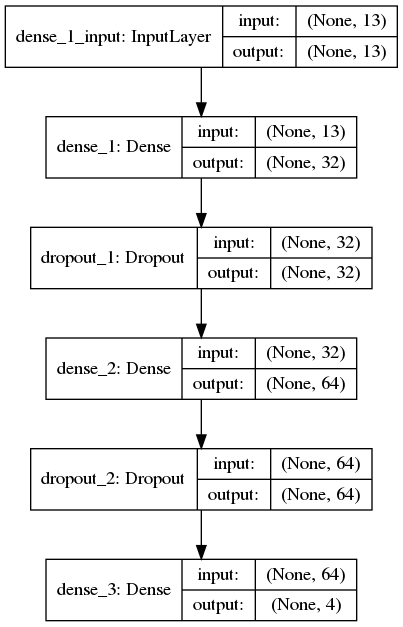
\includegraphics[scale=0.4]{images/Cm-Architecture.png}
    		\end{center}
    		\caption{Arhitectura rețelei (imagine produsă de Keras API)}
    		\label{fig:cm_arch}
    	\end{figure} 
    	
    	având urmatoarele straturi:
    	
    	\begin{itemize}
    		\item dense-1-input: reprezintă stratul input (unde 13 este numărul de coeficienți MFC obținuți cu ajutorul pachetului Librosa, specializat pe procesarea semnalelor audio);
    		\item dense-1: strat ascuns de 32 neuroni, cu funcția de activare ReLu;
    		\item dropout-1: un strat de tip dropout, care taie 0.2 (20\%) din conexiunile dintre straturi. Acest strat este utilizat cu rolul de a stimula rețeaua să învețe propagarea informației și în alte moduri;
    		\item dense-2: strat ascuns de 64 neuroni, cu funcția de activare ReLu;
    		\item dropout-2: un strat de tip dropout, care taie 0.2 din conexiuni;
    		\item dense-3: ultimul strat, care conține 4 neuroni (numărul de clase pe care dorim să le clasificăm). Uilizarea funcției softmax ne oferă probabilitatea apartenenței la fiecare clasă.
    	\end{itemize}
    	
    	\begin{figure}[H]
    		\begin{subfigure}[b]{0.45\textwidth}
    			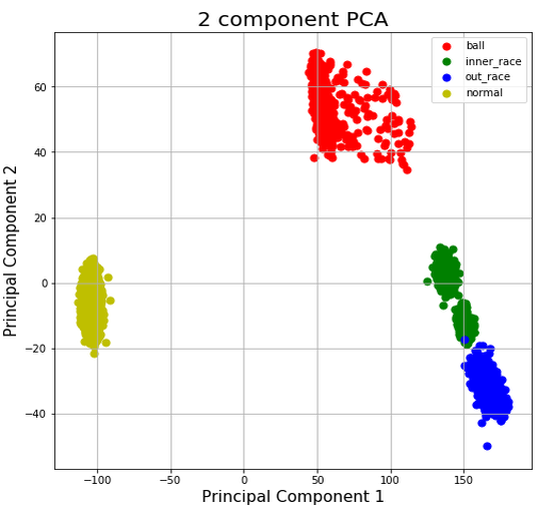
\includegraphics[width=\textwidth]{images/PCA_DE_12k_MFCC.PNG}
    			\caption{Plotarea coeficienților rulmentului DE}
    			\label{fig:DE_MFCC}
    		\end{subfigure}
    		\hfill
    		\begin{subfigure}[b]{0.45\textwidth}
    			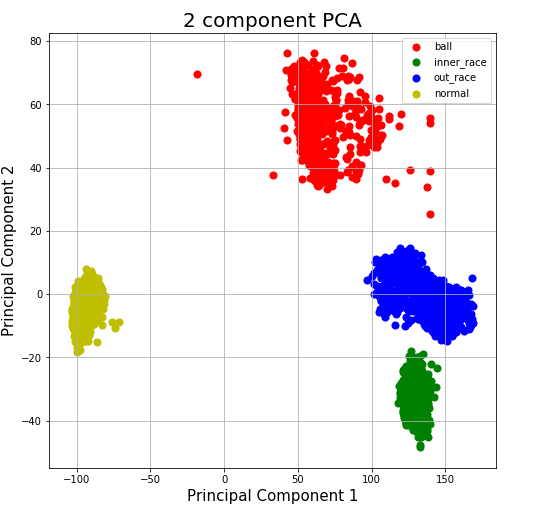
\includegraphics[width=\textwidth]{images/PCA_FE_12k_MFCC.PNG}
    			\caption{Plotarea coeficienților rulmentului FE}
    				\label{fig:FE_MFCC}
    		\end{subfigure}
    		\caption{Plotarea coeficienților}
    		\label{fig:DE_FE_MFC}
    	\end{figure}
    
    	Cu ajutorul tehnicii PCA (Principal Component Analysis), am reușit reducerea dimensionalității datelor. Din 13 coeficienți MFC, am compus 2 pe care i-am plotat, după cum se observă și în Figura \ref{fig:DE_MFCC}. Se poate vedea că este construită o adunare (cluster) pentru fiecare categorie de stare posibilă a rulmentului.
    	
    	\begin{table}[H]
    		\begin{tabular}{ |c|c|c|c|c|c| } 
    			\hline
    			Trained/Tested  & 0hp FE  & 1hp FE  & 2hp FE & 3hp FE & 0,1,2,3hp FE \\
    			\hline
    			0hp DE& 80.67\% 	& 85.45\%    & 83.11\%    & 84.13\%  & 83.14\% \\ 
    			\hline
    			1hp DE& 79.92\%    & 85.35\%    & 84.69\%    & 85.03\%  & 84.83\% \\ 
    			\hline
    			2hp DE& 79.89\%    & 83.03\%    & 82.15\%    & 82.28\%  & 84.63\% \\
    			\hline
    			3hp DE& 74.39\%    & 84.66\%    & 80.48\%    & 82.37\%  & 76.65\% \\
    			\hline
    			0,1,2,3hp DE& 79.97\% & 82.11\%    & 78.77\%    & 80.91\% & 83.71\% \\
    			\hline
    		\end{tabular}	
    		\caption{Antrenat pe rulmentul DE și testat pe pe rulmentul FE utilizând coeficienți MFC}
    		\label{tab:trainedDE_testedFE_differentLoads}
    	\end{table}
    	
    	Următorul pas a fost cel al antrenării rețelei, finalizarea experimentului venind cu rezultatele din Tabelul \ref{tab:trainedDE_testedFE_differentLoads}. Rezultatele ar fi putut fi mai bune, dar motivul principal al acestei precizii este dat de faptul că două clase sunt "inversate" între ele. Este vorba de inelul interior și inelul exterior. Acest comportament se poate observa și în Figura \ref{fig:DE_FE_MFC}. Culoarea verde reprezentată de cursa exterioară și culoarea albastră fiind cursa interioară sunt schimbate între ele în cadrul celor doi rulmenți. Acest comportament se poate explica datorită poziționării celor doi rulmenți. Nu reprezintă o problemă majoră, deoarece rețeaua este capabilă să clasifice aceste două stări de defecțiune de starea normală a unui rulment.
    	
    	Validarea modelului de învățare automată a venit odată cu rularea unor teste pe setul de date "NASA bearing set". După cum a fost menționat anterior, utilizând tehnici statistice, am putut afla perioada în care rulmenții încep să se strice. Testul a constat în predicția stării rulmentului până la momentul defecțiunii, precum și după. Rezultatele au fost promițătoare, modelul recunoscând în timpul intervalul de rulaj sănătos, rulmentul ca neavând nicio problemă din punct de vedere mecanică, iar în jurul perioadei de defectare, modelul determinând condiția rulmentului ca fiind una nesănătoasă.
 		
   \clearpage 	
   \section{Concluzii} 
   		Putem spune că utilizarea tehnicilor de procesare de semnal în domeniul învățării automate este o abordare inedită și foarte puțin exploatată. Cele mai populare tehnici de procesare de semnal (transformata Fourier pe terment scurt, coeficienții MFCC, crearea spectogramelor etc) au fost pârghiile în cadrul antrenării rețelor neurale.
   		
   		Cu aplicația Pianify am reusit să demonstrez două concepte: identificarea notelor și recunoașterea instrumentelor. Faptul că în cadrul unei melodii, putem identifica fiecare notă muzicală în funcție de frecvența emisă, captată cu ajutorul tranformatei Fourier pe termen scurt, a fost primul pas spre "încercarea" recunoașterii instrumentelor. Lipsa unui număr optim de date nu a fost un impediment major, deoarece am reușit cu ajutorul rețelelor neurale autoencoder generarea datelor sintetice destul de veridice inputului dat. Recunoașterea instrumentelor muzicale și separarea lor pe canale diferite a ajutat îndreptarea atenției și spre un domeniu mai industrial, cel al monitorizării condiției de funcționare a unui rulment.
   		
   		Efectuând o analiză asupra seturior de date utilizate în cadrul iterațiilor experimentale cu rulmenți, s-a reușit obținerea unui mod de antrenare independet de mărimea, numărul de bile și frecvențele emise de un rulment. Acest set de experimente au prins culoare în final prin publicarea unui articol: Bogdan Hanganu, Lucian Andrei Radu, Alexandra Băicoianu "Machine Learning For Condition Monitoring: Latest Trend And Review" în cadrul revistei științifice International Business Information Conference (35th "IBIMA"), Spain 2020.
   		
   		Însă, întotdeauna putem otimiza rezultatele obținute într-o aplicație, mai ales una care folosește învățarea automată. Îmbunătățirile care pot fi adăugate în aplicația Pianify se învârt în jurul rețelei neurale. Prin adăugarea unui număr mai mare de instrumente pe care am dori să le recunoască dar și o analiză mai profundă asupra frecvențelor, am fi obținut rezultate mai bune. În cazul monitorizării rulmenților, experimentul final pe care l-am dorit a fost acela de a testa modelul antrenat pe un caz real, prin achiziția datelor cu ajutorul unui senzor.
   \clearpage
   \printbibliography
   \clearpage
   %\lstlistoflistings
	\begin{figure}[H]
		\begin{center}
			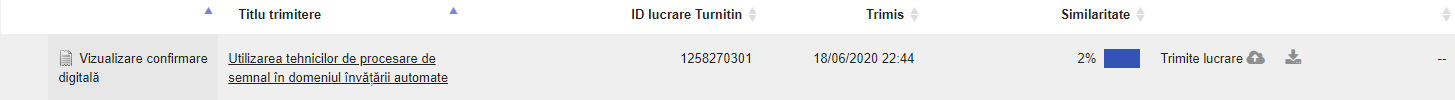
\includegraphics[scale=0.4]{images/plagiat.PNG}
		\end{center}
		\caption{Licență similaritate}
		\label{fig:sim}
	\end{figure} 	
\end{document}